\documentclass[a4paper,11pt,twoside,fleqn,openright]{memoir}
 
% Pakker
\usepackage[utf8]{inputenc} % Så må vi bruge æ, ø og å
%\usepackage[ansinew]{inputenc}
%\usepackage[danish]{babel} % Dansk opsætning
\usepackage[T1]{fontenc} % Hjælper med ordeling ved æ, ø og å. Sætter fontene til at være ps-fonte i stedet for bmp.
%\usepackage[scaled]{beramono} % Bedre monospace font
\usepackage{amsmath,amsfonts,amssymb} % God matematik
\usepackage{sistyle} % Enheder til fysik
\usepackage{array,booktabs} % Til gode tabeller
\usepackage{ragged2e} % For at kunnu lave tabeller med fast kolonnebredde, bruges sammen med 'array'
\usepackage{float} % Vi må nu bruge H som placering til floats
\usepackage{hhline} % Sum linie i tabel
\usepackage{multirow} % Fletning af rækker
\usepackage{multicol} % Fletning af kolonner
\usepackage{xcolor} % Vi kan bruge \color osv
\usepackage{colortbl} % Muligøre farver i tabeller
%\usepackage[danish=quotes]{csquotes} % Danske anførselstegn, brug enquote{}
\usepackage[english=british]{csquotes} 
\usepackage{graphicx} % Inkludere ekstern grafik
\usepackage[english,final]{varioref} % Vi kan anvende \vref
\usepackage{natbib} % Bedre litteratur henvisninger
\usepackage{pdfpages} % Inkludere en pdf side som en side  
\usepackage{acronym} % Smart akronymhåndtering
\usepackage{suffix} % Krævet af acronym
\usepackage{listings} % Til at inkludere kildekode direkte
\usepackage{lipsum} % Lorem ipsum dolar sit amet
\usepackage{caption} % Vi kan bruge \captionof
\usepackage{subfig} % Vi kan nu bruge \subfloat
\usepackage{calc} % Vi kan regne med tællere
\usepackage{changepage} % Vi kan ændre sidelayoutet lokalt
\usepackage{layout} % Vi kan se dimensionecne på vores layout med \layout
\usepackage[footnote,final,english,silent,nomargin]{fixme}
\usepackage[colorinlistoftodos]{todonotes}
\usepackage[pdftex,bookmarks=true,bookmarksnumbered=true]{hyperref} % Links i dokumentet
\usepackage{textcomp} % HVAD FANDEN GØR DENNE PAKKE?
\usepackage{threeparttable} % Så vi kan lave tablenotes (se latexbogen)
\usepackage{fixltx2e} % HVAD FANDEN GØR DENNE PAKKE?
\usepackage{minitoc} % Vi kan lave del inholdsfortegnelser forhåbentlig
\usepackage{enumitem} % Better lists
\usepackage{geometry}

% For sjov pakker
\usepackage{marvosym}
\usepackage{wasysym}
%\usepackage{fourier}

\captionsetup{font={small,sf},labelfont=bf}

\pagestyle{companion}

% Andre egensakber for komandoer
\newcommand\Cpp{C\raisebox{\height / 2}[\height][\depth]{\tiny ++}} % Pænere C++
\newcommand{\mimg}[4]{\marginpar{\small \centering{\includegraphics[width=#1]{#2}\captionof{figure}{\newline #3}\label{#4}}}} % Margin billede
\newcommand{\lmimg}[4]{\marginpar{\small\centering{% Latex margin billede
  \def\svgwidth{#1}
  \graphicspath{{illustrations/}}
  \input{illustrations/#2.pdf_tex}
  \captionof{figure}{\newline #3}
  \label{#4}}}
}
\newcommand{\mnote}[1]{\marginpar{\small \textsf{\textbf{Note}\\{#1}}}} % Margin note
\newcommand{\mcd}[1]{\marginpar{\textsf{\textbf{
\includegraphics[height=11pt]{frontmatter/media-optical}}\\\url{#1}}}} % CD-rom henvisning i margin
\newcommand{\cd}[1]{
\includegraphics[height=9pt]{frontmatter/media-optical}\url{#1}} % CD-rom henvisning i tekst
\newcommand{\limg}[5]{\begin{figure}[#1]
  \centering
  \def\svgwidth{#2}
  \graphicspath{{illustrations/}}
  \input{illustrations/#3.pdf_tex}
  \caption{#4}
	\label{#5}
\end{figure}}
\newcommand{\head}[1]{{\slshape{#1}}\vspace{5mm}} % Header
\newcommand{\tail}{\vspace{3mm}\fancybreak{$*\quad*\quad*$}\vspace{3mm}} % Røvhul
\newcommand{\enhed}[1]{\hfill\hbox{[#1]}\qquad} % At indsatte heb enheder i firkantparentes i "equation"
\newcommand{\dB}[0]{\hbox{dB}} % At skrive dB oprejst
%\addto\captionsdanish{
%\renewcommand\appendixname{Appendiks}
%\renewcommand\contentsname{Indholdsfortegnelse}

% Make vectors bold instead of a arrow
\let\oldhat\hat
\renewcommand{\vec}[1]{\mathbf{#1}}
\renewcommand{\hat}[1]{\oldhat{\mathbf{#1}}}

\makechapterstyle{box}{
  \renewcommand*{\printchaptername}{}
  \renewcommand*{\chapnumfont}{\normalfont\sffamily\huge\bfseries}
  \renewcommand*{\printchapternum}{
    \flushleft
    \begin{tikzpicture}[line width=4pt]
      \draw (0,1) -- (0,0) -- (1,0);
      \draw (2,1) -- (2,2) -- (1,2);
      \draw[color=gray] (1cm,1cm) node { \chapnumfont\thechapter };
    \end{tikzpicture}
  }
  \renewcommand*{\chaptitlefont}{\normalfont\sffamily\Huge\bfseries}
  \renewcommand*{\printchaptertitle}[1]{\flushleft\chaptitlefont##1}
  \setlength\beforechapskip{-100pt}
}

\newif\ifchapternonum
\makechapterstyle{nickoe}{
\renewcommand\printchapternonum{\chapternonumtrue}
  \renewcommand*{\printchaptername}{} % Removes the 'Chapter' text
  \renewcommand*{\chapnumfont}{\fontfamily{pbk}\fontseries{m} \fontshape{n}\fontsize{80}{35}\selectfont } % Does some magic
  \renewcommand*{\printchapternum}{}
  %\hfill 
  %\fontfamily{pbk}\fontseries{m} \fontshape{n}\fontsize{80}{35}\selectfont % Makes a gigantic number
  %\chapnumfont\thechapter} % Removes the 'Chapter's number
  \renewcommand*{\printchaptertitle}[1]{%
  \noindent%
  \ifchapternonum%
  \begin{tabularx}{\textwidth}{X}%
  {\parbox[b]{\linewidth}{\raggedright \hskip -0.6em \chaptitlefont ##1}%
    \vphantom{\raisebox{0pt}{\chapnumfont 1}}}
  \end{tabularx}%
  \else

  \begin{tabularx}{\textwidth}{Xl}
  {\parbox[b]{\linewidth}{\raggedright \hskip -0.6em \chaptitlefont ##1} }
  & \raisebox{0pt}{\raggedleft \chapnumfont \hskip -0.5cm \thechapter \hskip -0.5cm}%
  \end{tabularx}%
  \fi
  \hrule
  }

  %\flushleft\chaptitlefont##1} % Prints the chaptertitle
  %\renewcommand{\afterchaptertitle}{\par\nobreak\medskip\hrule\vskip\afterchapskip}
  \setlength\beforechapskip{-100pt} % Makes the chapter go up on the page

}

\newenvironment{ffk}[0]% formel forklaring
{\begin{list}{}%
         {\setlength{\leftmargin}{\mathindent}}%
         \item[]%
}
{\end{list}}

% Akronyms formatering
\renewcommand*{\acsfont}[1]{#1}
\renewcommand*{\acffont}[1]{#1}
\renewcommand*{\acfsfont}[1]{#1}

% Farve definitioner
\definecolor{shadecolor}{gray}{.95}

\lstloadlanguages{C,VHDL,Java}
% Kodeformatering [C]
\lstnewenvironment{ccode}[2][]{
  \def\lstlistingname{Source code}
  \lstset{
    language=C,
    escapeinside={(*@}{@*)},  % a line can set with: (*@\label{c:labelname}@*)
    keywordstyle=\bfseries,
    commentstyle=\color{blue}, 
    basicstyle=\ttfamily\selectfont\footnotesize,
    numbers=left,
    numberstyle=\tiny,
    tabsize=2,
    showstringspaces=false,
    backgroundcolor=\color{shadecolor},
    frame=lines,
    captionpos=b,
    caption={#1},
    label={#2}
  }
}{}

% Kodeformatering [VHDL]
\lstnewenvironment{VHDL}[2][]{
  \def\lstlistingname{Source code}
  \lstset{
    language=VHDL,
    keywordstyle=\bfseries,
    commentstyle=\color{blue}, 
    basicstyle=\ttfamily\selectfont\small,
    numbers=left,
    numberstyle=\tiny,
    tabsize=2,
    showstringspaces=false,
    backgroundcolor=\color{shadecolor},
    frame=lines,
    captionpos=b,
    caption={#1},
    label={#2}
  }
}{}

% Kodeformatering [Assembler]
\lstnewenvironment{asmcode}[2][]{
  \def\lstlistingname{Source code}
  \lstset{
    language=[x86masm]Assembler,
    keywordstyle=\bfseries,
    commentstyle=\color{blue}, 
    basicstyle=\ttfamily\selectfont\small,
    numbers=left,
    numberstyle=\tiny,
    tabsize=2,
    showstringspaces=false,
    breaklines=true,
    backgroundcolor=\color{shadecolor},
    frame=lines,
    captionpos=b,
    caption={#1},
    label={#2}
  }
}{}

% Kodeformatering [Java]
\lstnewenvironment{javacode}[2][]{
  \def\lstlistingname{Source code}
  \lstset{
    language=Java,
    keywordstyle=\bfseries,
    commentstyle=\color{blue}, 
    basicstyle=\ttfamily\selectfont\small,
    numbers=left,
    numberstyle=\tiny,
    tabsize=2,
    showstringspaces=false,
    breaklines=true,
    backgroundcolor=\color{shadecolor},
    frame=lines,
    captionpos=b,
    caption={#1},
    label={#2}
  }
}{}

% Kodeformatering [XML]
\lstnewenvironment{xmlcode}[2][]{
  \def\lstlistingname{Source code}
  \lstset{
    language=XML,
    keywordstyle=\bfseries,
    commentstyle=\color{blue},
    basicstyle=\ttfamily\selectfont\small,
    numbers=left,
    numberstyle=\tiny,
    showstringspaces=false,
    backgroundcolor=\color{shadecolor},
    frame=lines,
    morekeywords={msgid, repeat, mmsi, navstat, rot, sog, posaccu, lon, lat, cog, truehead, timestamp, manoeuvre, raim, commstate, utc_year, utc_month, utc_day, utc_hour, utc_min, utc_sec, txbcast, name, aisver, imo, call, cargo, a, b, c, d, fixdev, eta_mon, eta_day, eta,hour, eta_min, draught, dest, dte, spare},
    captionpos=b,
    breaklines=true,
    caption={#1},
    label={#2}
  }
}{}

% \part omdefinering, nu med beskrivende tekst
\def\descpart#1#2{
  \par\newpage\clearpage % Page break 
  \vspace*{5cm} % Vertical shift 
  \refstepcounter{part}% Next part
  %\addcontentsline{toc}{part}{\texorpdfstring{\rlap{\thepart}\hspace{1.2em}#1}{\thepart\ #1}} % Adds entry to TOC 
  \addcontentsline{toc}{part}{\texorpdfstring{\rlap{\thepart}\hspace{2em}#1}{\thepart\ #1}} % Adds entry to TOC 
  {\centering \textbf{\Huge Part \thepart}\par}
  \vspace{1cm} % Vertical shift
  \thispagestyle{chapter} % Gives the pagestile an the memoir chapterpagestyle
  {\centering \textbf{\Huge #1}\par}
  \begin{center}
  {\parbox{9cm}{
  \vspace{2cm} % Vertical shift
  \noindent \slshape{#2} % Some text
  }}
  \end{center}
  \vfill\pagebreak % Fill the end of page and page break
}

%------------
\def\appendixpart#1#2{
  \par\newpage\clearpage % Page break 
  \vspace*{5cm} % Vertical shift 
  \addcontentsline{toc}{part}{\texorpdfstring{\rlap{\thepart}\hspace{2em}#1}{\thepart\ #1}} % Adds entry to TOC 
  \thispagestyle{chapter} % Gives the pagestile an the memoir chapterpagestyle
  {\centering \textbf{\Huge #1}\par}
  \begin{center}
  {\parbox{9cm}{
  \vspace{2cm} % Vertical shift
  \noindent \slshape{#2} % Some text
  }}
  \end{center}
  \vfill\pagebreak % Fill the end of page and page break
}


%------------

% At bruge figurer der fylder mere end brødteksten
% Der defineres nogle ekstra længder
\newlength{\fullwidth}
\setlength{\fullwidth}{\textwidth}
\addtolength{\fullwidth}{\marginparsep}
\addtolength{\fullwidth}{\marginparwidth}
\newlength{\fullmargin}
\setlength{\fullmargin}{\marginparwidth}
\addtolength{\fullmargin}{\marginparsep}
% For at bruge det, skal man f.eks. gøre således:
%\begin{figure}[h]
%\begin{adjustwidth*}{-\fullmargin}{}
%\includegraphics[width=\fullwidth]{./sti}
%\end{adjustwidth*}
%\caption{Beskrivelse her}
%\laber{fig:label}
%\end{figure}

% \degC for grader C
% \arcdeg for gradtegn
\renewcommand{\epsilon}{\varepsilon}
\newcommand{\MATLAB}{M{\footnotesize ATLAB}}
\parindent 8pt

% Orddeling
% Ord der deles forkert kan skrives her, men bindestreg ved stavelser og mellemrum mellem ordene
\hyphenation{ar-bejds-in-ten-si-ve an-grebs-vink-ler ind-gangs-im-pe-dans ro-ta-ti-ons-en-ko-der deres clock-fre-kvens sys-tem-et na-vi-gate} 

\hypersetup{
  pdftitle={Formation Control for Unmanned Surface Vehicles for Surveying Purposes},
  pdfsubject={Master's thesis, Aalborg University},
  pdfauthor={Nick \O stergaard and Jeppe Dam},
  pdfcreator=LaTeX rules for typesetting!,
  linkcolor=black,
  citecolor=black,
  filecolor=black,
  urlcolor=black
}


% This can be used to reduce the number of chapters to be formatted
%\includeonly{ros}

\begin{document}
\frontmatter
% Frontpage
\newgeometry{left=3cm,top=3cm,right=3cm,bottom=3cm}
\author{Jeppe Dam and Nick Østergaard}
\title{\textbf{\emph{Formation Control of Autonomous Surface Vehicles for Surveying Purposes}}}
\date{\today}
\maketitle
\thispagestyle{empty}
\begin{center}
	\includegraphics[width=13cm]{frontmatter/aauship}
\end{center}
\vfill
\begin{center}
	
\includegraphics[width=5cm]{frontmatter/AAU_LOGO_CMYK_UK}\\
	Department of Electronic Systems
\end{center}
\clearpage
\restoregeometry


%\chapterstyle{nickoe}
\cleardoublepage
\thispagestyle{empty}
\newgeometry{right=2cm}
\noindent
\begin{minipage}[l]{0.50\textwidth}
	\centering
	
\includegraphics[width=3.35cm]{frontmatter/AAU_LAT_CIRCLE_blue_rgb}
\end{minipage}
\begin{minipage}[r]{0.50\textwidth}

\noindent
	\begin{tabular}{l}
		{\textsf{\small \textbf{Institute of Electronic Systems}}}\\
		{\textsf{\small \textbf{Control Engineering}}} \\
		{\textsf{\small Fredrik Bajers vej 7}} \\
		{\textsf{\small 9220 Aalborg \O st}} \\
		{\textsf{\small Phone 99 40 86 00}} \\
		{\textsf{\small http://es.aau.dk}}
	\end{tabular}
\end{minipage}


%\fbox{
\begin{minipage}[c]{0.45\textwidth}
	\begin{description}[leftmargin=\parindent+0.5em,labelindent=\parindent]
	\item [\textbf{Title:}] \tightlist
	\item Formation Control of Autonomous Surface Vehicles for Surveying Purposes
	\end{description}

	\begin{description}
	\item [\textbf{Theme:}] \tightlist
	\item Master’s thesis
	\end{description}

	\begin{description}
	\item[Projectperiod:] \tightlist
	\item 2014
	\end{description}
	%  \hspace{4cm}
	\begin{description}
	\item[Projectgroup:] \tightlist
	\item 1034
	%  \hspace{4cm}
	\end{description}

	\begin{description}
	\item[Participants:] \tightlist
	\item Nick \O stergaard 
	\item Jeppe Dam
	\end{description} 

	\begin{description}
	\item[Supervisor:] \tightlist
	\item Jesper Abildgaard Larsen
	\end{description}

	\begin{description}
	\item[Number of printed copies:] 2
	\item[Number of pages:] \arabic{lastsheet} 
	\item[Appendices:] ??\todo{update} + website
		\footnote{Website with additional material, \url{http://kom.aau.dk/group/14gr1034/attached}}
	\item[Finished on:] \today
	\end{description}
\end{minipage}
\hfill
\begin{minipage}[r]{0.50\textwidth}
	{\textbf{Synopsis:}} \\
	\fbox{\parbox[c]{\textwidth-0.5em}{
	\bigskip
	{\vfill{\small \lipsum[1]

	\bigskip}}
    }}
\end{minipage}
%}
\vfill
\begin{center}
	
\includegraphics[width=1.35cm]{frontmatter/ca-logo.pdf}
\end{center}
\restoregeometry

%Rapporten skal afleveres til følgende:
%1 stk. til hovedvejlederen (afleveres til studiesekretæren)
%1 stk. til censor (afleveres til studiesekretæren)
%1 stk. til hver studerende i gruppen

\chapter{Preface}
\todo[inline]{This has to be written some time in the future, describe what this doc is.}

\subsubsection*{Thanks to}
\todo[inline]{Say thanks to someone, Aalborg Havn if they are helpfull? Karl D. has been glad to answer ROS related questions.}


\begin{center}
  \begin{minipage}[t]{0.47\textwidth}
    \centering \vspace{1.5cm} \hrule \vspace{1mm} Nick \O stergaard
  \end{minipage}
  \hfill
  \begin{minipage}[t]{0.47\textwidth}
    \centering \vspace{1.5cm} \hrule \vspace{1mm} Jeppe Dam
  \end{minipage}
\end{center}


\newpage
\section*{Reading guide}
The following report is divided into parts, related to different phases of the project. The parts are divided into chapters, the chapters describe different aspects of the project. The chapters are subdivided a number of times to further split up the content into specific topics. The report is ended with an appendix part, that contains all the material that is relevant to the project, but not necessarily interesting to the reader, such as measurement journals and transcripts of meetings.

\begin{description}
\item[Citations] in the report is done according to the Harvard method, the list of references can be found \vpageref{ch:litt}. The elements on the list of references are sorted by author.
\item[Acronyms] are written to their full extend, the first time they are used, with the acronym in parentheses, thereafter only the acronym is used. The list of acronyms can be found \vpageref{ch:acronyms}.
\item[Notation] of vectors are written in bold font with lower case letters ($\vec{v}$), matrices are written in bold font with upper case letters ($\vec{M}$). Single variables and constants are typeset in normal math ($x$).
\item[Attached] to the report is a CD, which contains copies of web references and other digital files (source code, scripts and raw measurement data) that could be of interest to the reader. In some places in the report there will be a reference to the CD; this will look like this: \cd{/path-to-file}.
\end{description}


\cleardoublepage
\tableofcontents
\printnomenclature
\chapter{Acronyms}
\label{ch:acronyms}
\begin{acronym}[TDMA]
%\begin{acronym}[HBCI]
	\acro{AAU}{Aalborg University}
  \acro{ASV}{Autonomous Surface Vessel}
	\acro{ADC}{Analog to Digital Converter}
  \acro{AHRS}{Attitude and Heading Reference System}
  \acro{BODY}{The body frame}
  \acro{CFD}{Computational Fluid Dynamics}
  \acro{DOF}{Degrees-Of-Freedom}
  \acro{DP}{Dynamic Positioning}
  \acro{ECEF}{Earth-Centered Earth-Fixed} 
  \acro{ECI}{Earth-Centered Inertial}
  \acro{EKF}{Extended Kalman Filter}
  \acro{FRF}{Formation Reference Frame}
  \acro{FRP}{Formation Reference Point}
	\acro{GNC}{Guidance, Navigation and Control}
  \acro{GNSS}{Global Navigation Satellite System}
  \acro{GPS}{Global Positioning System}
  \acro{GRS}{Ground Segment}
  \acro{HLI}{High Level Interface}
  \acro{IMU}{Inertial Measurement Unit}
	\acro{IP}{Internet Protocol}
	\acro{IPv4}{Internet Protocol version 4}
	\acro{IPv6}{Internet Protocol version 6}
  \acro{KF}{Kalman Filter}
  \acro{LKF}{Linear Kalman Filter}
  \acro{LOS}{Line-Of-Sight}
  \acro{LLI}{Low Level Interface}
	\acro{LSB}{Least Significant Bit}
  \acro{LTI}{Linear Time Invariant}
  \acro{MARG}{Magnetic, Angular Rate, and Gravity}
  \acro{MMSE}{Minimum Mean Square Error}
  \acro{MUV}{Multiple Unmanned Vehicle}
  \acro{MPC}{Model Predictive Control}
  \acro{NED}{North-East-Down}
  \acro{OSM}{OpenStreetMap}
  \acro{PWM}{Pulse Width Modulation}
  \acro{ROS}{Robot Operating System}
  \acro{RTK}{Real Time Kinematic}
  \acro{SOG}{Speed Over Ground}
  \acro{SSS}{Single Screw Ship}
  \acro{SSM}{State Space Model}
  \acro{TSS}{Twin Screw Ship}
  \acro{UGAS}{Uniformly Globally Asymptotically Stable}
  \acro{UGES}{Uniformly Globally Exponentially Stable}
  \acro{UGS}{Uniformly Globally Stable}
  \acro{UKF}{Unscented Kalman Filter}
  \acro{WGS84}{World Geodetic System 1984}
\end{acronym}



\mainmatter
\descpart{System design}{All the magic about the system}
\chapter{Introduction}
\head{In this chapter is the motivation for the project stated and the previous work within the subject will be summed up.}

\section{Motivation and the AAUSHIP Project}
The Port of Aalborg would like Aalborg University to help them to expand their options of improving the conditions of the Limfjord. One of their tasks is to map the seabed of the Limfjord to get bathymetry data. This will help them guide larger cargo ships to port while using the autonomous ships as guidance.

Another aspect from The Port of Aalborg is a task to escort larger ships with cargo into The Port of Aalborg. This is done by a pilot whom needs to sail out to incoming larger cargo ships and escort them safely into port. The pilot does this in a pilot boat which is controlled manually by the pilot. The Port of Aalborg would like this process to become autonomous such that an autonomous boat can sail to the cargo ship and to some extend take over the control and guide the cargo ship into port. The system to do this implies that The Port of Aalborg needs an autonomous ship which can perform this task.

The mapping itself can be done by one ship or by more. For the moment one of the ships from The Port of Aalborg, which is manned, and covers the mapping of the closer part of the Limfjord ($\approx$ 65 km). This is only done every third year, but mapping around Hals Barre (a sandbar \todo{slet efterfølgende kommentar igen engang}and not a beach bar) at the end of the Limfjord is a more critical place and is mapped every third month.

If The Port of Aalborg had an autonomous ship fleet at their disposal, which could sail out and do the mapping autonomously, they would get updated bathymetry maps with a higher update frequency than they have currently \citep{portofaalborg}. This will result in a digitalizing of the seabed, a digital map, which has different implementation options by The Port of Aalborg.

This thesis will utilise formation control and extensions to manoeuvre agents through a specified area for surveying purposes. The aspect of formation control is chosen due to the rather large areas that The Port of Aalborg needs so cover. When applying formation control it is assumed to be faster to cover a larger area than if one single boat needed to scan the area. The formation that are to be chosen depends on the specific area of interest, which could e.g. be inside the harbour or around the pillars of the bridge. Chapter~\vref{ch:formcontrol} will introduce what kind and scopes of formation control that exists today. These theories makes the basis for the formation control within the scope of this project.

As a future scope this can be used when making a model of the seabed of how this will get sanded. This model can tell The Port of Aalborg when to go clean the seabed. The AAUSHIP project can be used to verify this model, such that The Port of Aalborg do not have to go out with equipment to solve the sanding without the need of it.

\section{The Mission}
\label{sc:mission}
Within the scope of this project the robots will be unmanned ships,
\ac{ASV}. The ship's main purpose will be to map the seabed by using
sonars to obtain bathymetry data. When one ship need to do this alone, and due to the range of
the sonar, the time spend could be improved by using multiple ships. The sonar scanning would
be done as seen on figure~\vref{fig:concept-art}.

\begin{figure}[htbp]
	\centering
	\subfloat[One ship\label{fig:concept-art1}]{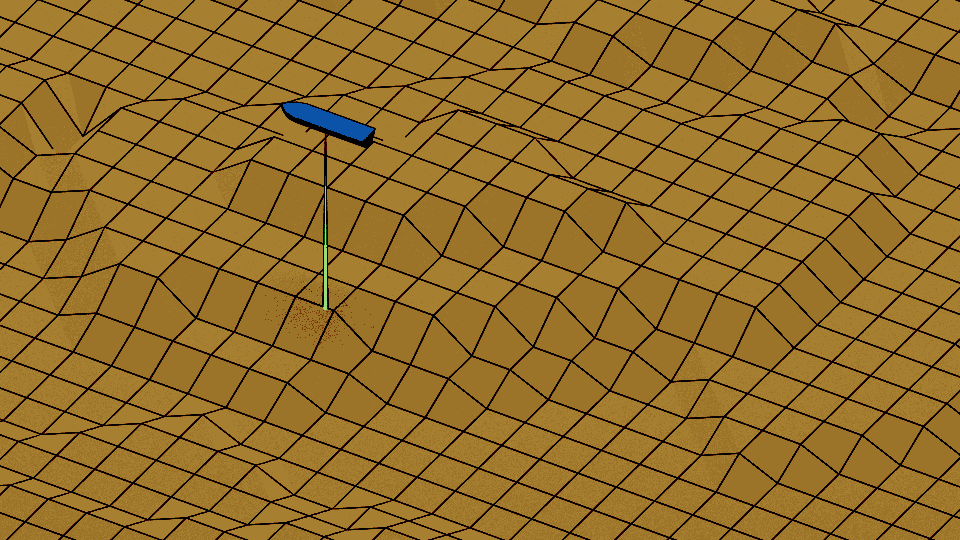
\includegraphics[width=0.48\textwidth]{fig/conseptart-single}}
	\ % One forced space to seperate figures
	\subfloat[Thee ships\label{fig:concept-art3}]{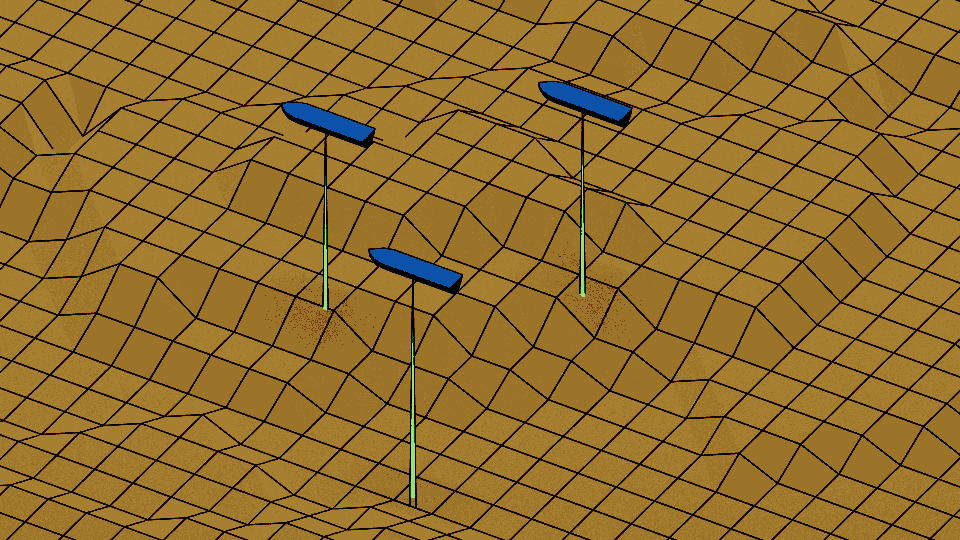
\includegraphics[width=0.48\textwidth]{fig/conseptart-formation}}
	\caption{Comparison of two ways to cover an area with a lawn mower
	pattern.}
	\label{fig:concept-art}
\end{figure}

When only one ship (figure~\vref{fig:concept-art1}) need to map a complete seabed this process could
take up much time dependent on the area that need to be covered. The
time spend could be improved to make this mapping more efficient. One
way of optimizing the time used is to add more ships (figure~\vref{fig:concept-art3}) to help map the
seabed. To make the process of this as optimal as possible it could be
of benefit to implement formation control in the specific assignment.

I cooperation with the port of Aalborg, a use case is presented, where we can perform tests of the platform, and use those to compare the performance of our system to their system.
\begin{figure}[htbp]
	\centering
	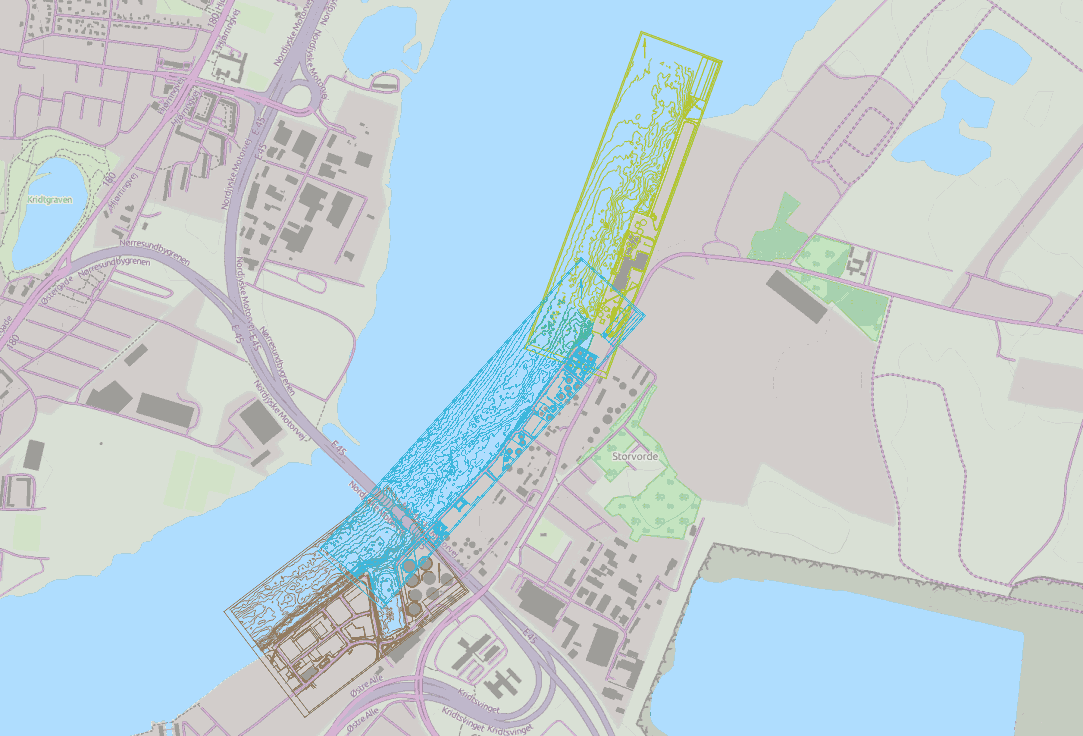
\includegraphics[width=\textwidth]{fig/use-case-data}
	\caption{Area of the harbour at Aalborg Portland provided as sample
	data from Aalborg Havn. Background map data CC BY-SA OpenStreetMap.}
	\label{fig:diffforms}
\end{figure}

When performing this kind of surveying with multiple ships, it is important to take note of the kind of sensor it uses and the coverage that it provides. Initially the port of Aalborg used single beam echo sounders, but have in recent years turned over to multibeam sonars for their survey boat, which has improved their resolution and time for a survey. But they still wishes to improve the survey update rate, by e.g. using fairly low cost autonomous ships to get better indication of the seabed to identify if an expensive thorough survey is needed. An image of the survey vessel they use now used can be seen on figure \ref{fig:alba}. As it can be seen, this survey vessel is relatively large, being over 20 metres long. To comparison is the AAUSHIP only 1.1 metres long. For surveying in smaller areas, like inside the harbour area, Aalborg Havn uses a smaller scale vessel which is 12 metres long. This vessel is only used at the smaller areas thus not the one being used out in the Limfjord close to Aalborg.
\begin{figure}
	\centering
	\includesvg{alba}
	\caption{The survey vessel used by Aalborg Havn named Alba.}
	\label{fig:alba}
\end{figure}



%This could be done in several ways, but is mostly thought of in a
%rigid formation, such that the formation maps the same area of the
%seabed the whole time. The idea can be seen on
%figure~\vref{fig:concept-art}.
 % Talk specifically about the data from havnen?
\chapter{General formation control}
\head{This section will give a short introduction to formation control in general, by discussing existing formation control paradigms and relating them to the motivation of the AAUSHIP as a survey platform consept.}

%\head{Formation control in general is concerned with simultaneous control of dynamic systems. These systems is often referred to as agents where the objective of these is to maintain a static reference to a specified object. This object could be another agent witch then would be referred to as the leader. The other agents objective will then be to stay in the relative position to the leader within a static formation.}

The theory of formation control in general is widely applied. It is usually applied in assignments regarding control of robots which needs to be placed relative to each other. Depending on the given task of the robots, and which type of robots are in focus, the formation can be utilized in different ways \cite{muv-survey1}.

The robots can also be of various types: Driving vehicles, helicopters, aeroplanes, ships etc. which can be both manned and unmanned. The tasks that these robots needs to fulfill can vary greatly. Robots in groups in general have many purposes such as vacuum cleaning robots, who needs to clean a rather large area or flying swarm robots like quadcoptors who can make different kinds of assignments. When quadcoptors work as a combined group they could lift a certain amount of payload to achieve their goal as a group, or they could work individually in a network to do several smaller tasks. An example of how quadcoptors are working together can be examined at \citep{ethswarm}.

All the robots in the terminology of \cite{muv-survey} are called \textit{agents}. These agents move either individually or in formation. This formation can be rigid or be flexible. If the agents move in rigid formation they will keep their relative positions to each other and must not diverge from the formation. The formation could also be flexible which sometimes is preferable. If the distances between three agents on line are large, and an obstacle needs to be avoided, only one of the agents needs to move from this obstacle if the formation is flexible. This can be seen on figure~\vref{fig:form_avoid_right}.
\begin{figure}[htbp]
	\centering
	\includesvg[width=0.5\textwidth]{form_avoid_right}
	\caption{A flexible formation where the right agent avoids an obstacle.}
	\label{fig:form_avoid_right}
\end{figure}

\section{State of the art}
When looking into formation control many different types of control can be taken into control. The main types of formation control are separated into six different types, separated by \cite{muv-survey}, all under the main topic \textit{multiple vehicles coordination strategies}. The overview for this can be found in the survey paper \cite{muv-survey} who explains the six main types and a few alternations of these.

The theoretical views on control of \ac{MUV}'s behaviour are by \cite{muv-survey} divided into two classes; centralized and decentralized systems. If the system is centralized this means that all control of the formation is done on one agent, and the others receive information from the core agent. This form of system has the advantage that the core agent can optimize vehicle coordination, accommodate individual agent faults and monitor the accomplishment of the mission. The main disadvantage of this system is that if a fault should occur in the core agent this will affect and facilitate a failure of the whole system.

The opposite way of controlling the system would be in a decentralized way. This way of controlling the formation is inspired by the aggregation of birds and fish. This makes each agent able to communicate and share information in between. This means that each agent is given its own part of the complete objective and thus can only complete a part of it, like moving around an object to get to end point of a trajectory. The advantage is that faults in a single agent can be overlooked, thus more robust to faults, but can result in a less efficient objective outcome. A decentralized system may be more appropriate to scale up such that more agents can be included and the computational load can, in difference from the centralized system, be split up onto more agents.

The different types of coordination and control algorithms within centralized and decentralized systems include: \textit{behavioural-based}, \textit{virtual structure}, \textit{leader-follower}, \textit{graph-based} and \textit{potential field approaches}. Within these structures are the terms \textit{cooperation control} and \textit{formation control} used. Cooperative control focuses on the global task that the group of agents needs to fulfil, and the formation control is the actions performed by each agent which is shared with the other agents in the group. 
\begin{description}[style=nextline]
	\item [Virtual structure]
	In a virtual structure is the entire formation treated as a single entity. The behaviour coordination for a group of agents in a virtual structure is uncomplicated compared to the coordination of many agents, due to the making of one structure e.g. based on fixed distances between the agents. The disadvantage falls on the centralization due to the structure treated as a single entity. If a failure in this structure happen results in a failure in the entire structure.
	\item [Behaviour Based Methods]
	The behavioural based model employs several behaviours for each of the agents and the final control used to control the formation is derived from a weighting of the relative importance of each of the behaviours. This could for instance be navigational behaviours to enable a navigation to be the main goal while avoiding hazards and stay in formation. So if one agent needs to avoid a collision with an obstacle the rest of the group should not take this into account. Only that single ship needs to leave the formation and get back into formation again.
	\item [Leader-Follower Approaches]
	Applying leader-follower methods designates one agent as being the leader and the rest of the agents as followers. The following agents need to position themselves relative to the leader and maintain a desired relative position to the leader. This makes the simplicity to this method, but there is no feedback from the followers to the leader and thus makes that a disadvantage. Separation-separation and separation-bearing are two popular leader-follower formation controls, where the followers stay at specified separation and bearing from their designated leader. Within this method it is possible to split the group up into several smaller groups with their individual designated leader.
	\item [Potential Field Approach]
	Potential field approaches assigns potentials to agents to make a weighting between them. This weighting could for instance determine the relative distances between the agents. This is usually used when following a virtual leader, such that this process is only made relative to the agents within the structure. This method can make ensure a collision free formation when every agent has been assigned their potential weighting respectively. In this method obstacles can be included and have assigned potentials as well. This will become an avoidance radius from the specific object.
	\item [Graph Theory Approaches]
	When applying the graph theory method one assign every agent as a node and assign connections between the nodes. In graph theory this is denoted vertices and edges. The study with graph theory is mainly concentrated of the formation itself and related to changes within the structure. This can be related to the structure within a tree-structure which is used when assigning the formations in graph theory manor. This can be applied as communication analysis for the agents and consensus analysis can be of benefit. The edges between the nodes symbolizes the possible connections thus communication between them. The nodes that are connected are denoted as neighbours and are capable of communicating.
\end{description}

\subsection{Approaches on formation control}
When performing this kind of surveying with multiple ships, it is important to take note of the kind of sensor it uses and the coverage that it provides. Initially the port of Aalborg used single beam echo sounders, but have in recent years turned over to multibeam sonars for their survey boat, which has improved their resolution and time for a survey. But they still wishes to improve the update rate, by i.e. using fairly low cost autonomous ships.

\missingfigure{Picture of the port of Aalborg's survey boat.}

This does not have any relevant impact of how the mappings of the seabed would be due to the subsequent processing of the collected data from the maps.

Different formations of ships can be seen on figure~\vref{fig:diffforms}.
\begin{figure}[htbp]
	\centering
	\includesvg[width=0.5\textwidth]{diffforms}
	\caption{Different formations which the \ac{ASV}s can make.}
	\label{fig:diffforms}
\end{figure}

The formation of the ships may not need to be strictly rigid. Situations could appear where it would be of benefit to change the ship's formation. If the formation need to avoid an obstacle and one or more ships needs to go faster or slower, which leads to a change in the formation, it might be of benefit to regroup the formation which is faster to reach. An example can be seen on figure~\vref{fig:avoid}.

\begin{figure}[htbp]
	\centering
	\includesvg[width=0.5\textwidth]{form_avoid}
	\caption{A formation needs to go around an obstacle where the inner most ship chooses the shortest path and the formation regroups.}
	\label{fig:avoid}
\end{figure}

When doing the formation control it is important to figure out what one
want to achieve, and depending on the strategy and the formation type
some things are to be considered as requirements regarding how the
formation should work. In this discussion lawnmower patterns are considered. In this work thee ships are considered for simplicity, but it should be extensible to n-number of ships. The lawnmower patterns will suit well for the mapping of a seabed where one or more ships are to sail from shore to shore in a fjord.

\subsubsection{Initialisation}
When looking at the specific task several things needs to be taken into account. When starting the mission, the ships may start at positions that is not in the desired formation. It might be of importance that the ships are in
formation when they start tracking the desired track. Therefore some
attention must be given on how to make the ships initialize this
formation. This is referred to as the group coordination task. An approach is to make the ships sail individually to the
starting positions with a speed that makes them hit their respectively starting points at
the same time. If one reaches its start point much earlier
than the other it must stop, which is not wanted because it then can
drift out of position again. This basically means that there exists an initialization
phase and a tracking phase. The start heading should of
course align with the path at the start point such that the path following can begin with zero error. The ships could also target their group formation before starting at time zero at the path. This will eventually make the initialization take longer time but ensure that the ships have made the group coordination task and are ready to start at the path.

Another issue to be considered is to ensure that no ship at
any point in time reaches a minimum speed that is necessary for the
ship to not drift out of formation. This could be a problem in corners
of the formation if a stiff construction, where the inner most ship
has to move slower, to accommodate the shorter distance on an inner
circle arc.

Faults like blackout on a ship could also be considered in the control
design. I.e. what happens with the formation when one ship faults in a
blackout. Should the rest of the formation stop, should the formation
still follow this drifting ship or should the mission simply terminate
when it is discovered that a ship has blackout. This is under the assumption that the formation is decentralized and every ship has its own control and is not controlled from a mother ship.

In the initialization phase it is also relevant to consider how the
ships should avoid each other if they are on the wrong side of each
other. If it is of benefit that a specific ship is at the most inner route, and is located at an outer position before the group coordination, this ship needs to cross the formation to get to the desired starting position. This initialization needs to be adjusted in the initialization phase to ensure that no ships collide.

\begin{figure}[htbp]
	\centering
	\includesvg[width=0.4\textwidth]{cornoring}
	\caption{Two ships initializing and following the path offset
		equally on each side, ships are constrained to sailing parallel
		and heading the same as path when projected onto the path. Blue
	dot is start of path. Fully drawn splines is initializing phase.}
	\label{fig:cornoring}
\end{figure}

On figure~\vref{fig:cornoring} is a simple path following performed
with two ships in a stiff formation with an equal distance from the
path. It illustrates four steps. In step \#0 the ships initializes a
random position near the start of the path being the group coordination task. At \#1 it is tracking the
path in formation, whilst still in formation. This is referred to as a formation coordination task. At \#2, the green
(right) ship is in a tight inner curve where it is important to
consider design of the path such that the capabilities of the ship is not
exceeded to stay in formation. At \#3 it is back to straight line path
following in formation. \citep{thorvaldsen}.

\begin{figure}[htbp]
	\centering
	\includesvg[width=0.6\textwidth]{form_rigid_90}
	\caption{Three ships in formation needs to make a 90\textdegree turn and stays in their relative positions and keeps the rigid formation.}
	\label{fig:form_rigid_90}
\end{figure}

When the ships needs to make a turn about something they can do it in many ways. On figure~\vref{fig:form_rigid_90} the ships keep their formation whilst turning about the object. When they reach the other side and have finished their turn, the ships have kept formation but the outer most ship has now become the inner most ship. The reason to turn like this could be that the inner most ship, the yellow ship, cannot turn as sharp as demanded to stay the inner most ship. Therefore, instead of turning the formation, they stay geometrically rigid.

\begin{figure}[htbp]
	\centering
	\includesvg[width=0.6\textwidth]{form_change_90}
	\caption{Three ships in formation needs to make a 90\textdegree turn and changes their relative positions.}
	\label{fig:form_change_90}
\end{figure}

As seen on figure~\vref{fig:form_rigid_90} the ships could have benefit of turning like this. This way of turning could cause trouble in the top of the turn, where the ships eventually will collide due to errors and the relative close distance to each other. This way could be altered a little such that the ships will turn like on figure~\vref{fig:form_change_90}. There the ships adjust their position and velocities to ensure that they will not collide, but they will therefore leave their formation shortly to return back into position again.

\subsubsection{Degree of Actuation}
The degree of actuation is a matter that sets some limitations on how
the path following can be made, and thus the methods available to
control the ships.

AAUSHIP is a ship, which means that is is not fully actuated in the
whole 3D space, but this is not needed since it is moving on a
surface. To be fully actuated it must be able to have controls for
surge, sway and yaw.

There are different ways of controlling, and a few could be:
\begin{description}[style=nextline]
	\item [Three or more controls]
	When having three or more control parameters it is said that the vessel is fully actuated. This way of controlling is usually used in low-speed manoeuvring and stationkeeping mostly by offshore \ac{DP} vessels.
	\item [Two controls and Trajectory-Tracking control]
	Trajectory-Tracking is done in a three \ac{DOF} system, $e(t)\in\mathds{R}^2\text{X}S$. It is done with two control inputs, $u(t)\in\mathds{R}^2$. This means that the control problem is underactuated which cannot be solved by linear control theory. A vessel under these terms is able to manoeuvre along a path with constant sideslip angle using only surge and yaw. This is the classic approach for path following.
	\item [Two controls and Weather-Optimal heading]
	When taking the weather conditions, and in general the environmental disturbances, into account, it is done as a mean of all the disturbances. This is used to stabilize the vessel regarding the position. It is done by making the heading depend of the change in the mean of the environmental disturbances.
	\item [Two controls and Path-Following control]
	The standard way by having two controls, being surge and yaw, and achieving path-following, is to define a 2-D workspace. This workspace is placed along the trajectory with along-track and cross-track vectors that are to represent the error to minimize. This is usually done by applying the \ac{LOS} path following controller that makes use of surge and yaw to accomplish the path following. This implies that a six \ac{DOF} system model needs to be internally stable such that only the two control inputs are used.
	\item [One control]
	This is only done with systems with three \ac{DOF} and is normally only used to stationkeeping.
\end{description}
\citep{fossen}

\subsection{Delimitations}
Within the scope of the AAUSHIP project will the focus be to apply and extend a leader-follower approach at the ships. This will include several tasks. The two main tasks will be to make a group coordination task and a formation coordination task. The group coordination task will be, as described earlier, an objective to get the ships into the desired formation before or exactly at the starting point of the path following. The formation coordination task will be to make a leader, virtual or not, follow a predetermined path set by waypoints. The path should be generated from waypoints placed on a map due to that the ship needs to travel over larger distances. This will make a waypoint based follower where the path will be generated between the placed waypoints.

The placement of the waypoints will be placed such that the ships need to surge along a lawnmower pattern, where the turns have a lower requirement of turn radius dependent on the surge velocity of the most inner ship. This is due to the drift if the inner ship looses too much velocity.

When applying the leader-follower approach it needs to be determined how the formation precisely should be set up. In this project is only one leader considered at a time. The rest of the ships will act as followers to the leader. The idea can be seen on figure~\vref{fig:l_f} where only one leader is represented with a single or more followers.
\begin{figure}[htbp]
	\centering
	\includesvg[width=0.6\textwidth]{lead_follow}
	\caption{A leader is always assigned and potential followers are following.}
	\label{fig:l_f}
\end{figure}
When the followers are in formation with the leader is only the leader who is following a specified trajectory. The other ships, the followers, only keeps their position relative to the leader. This makes the predetermined formation moving along the path relative to how the leader is following the path. The leader is autonomous as well as the followers, but the path following is only done at the leader and the followers maintains their relative positions to the leader.

If the leader diverges from the path, drifting to the left, this will result in the whole formation drifting to the left. This problem can be dealt with in different ways, e.g. the control could react fast enough to make the formation get back on track within a specified time, or some fault tolerance could be done from the whole system. If the leader diverges from the path it could make the formation stay at their respective headings within a time slot before actuating towards the leader.

The formation needs to take into account if it is of benefit to change leader. If some kind of obstacle makes the formation turn about it, it might come to benefit to change the leader which needs to be done on the fly. This entails a change in the group coordination and the ships needs to set their relative position and heading from another ship.

The configuration of the formation will be set up, as a start, with one leader and a single follower. The follower will be offset from the leader with a distance of five metres. This can be seen on figure~\vref{fig:l_f1}.
\begin{figure}[htbp]
	\centering
	\includesvg[width=0.4\textwidth]{lead_follow1}
	\caption{The leader with a follower offset by 5 metres radius.}
	\label{fig:l_f1}
\end{figure}
This will be a rigid formation that the ships needs to keep at all times. The change of leader will eventually be taken into account when the ships needs to turn. If the formation needs to turn clockwise about it might be of benefit to change the leader. 

The location to test and implementation the AAUSHIPs will be in the Limfjord. The optimum will be to make the formation go across the Limfjord and back in lawnmower pattern and make measurements of the seabed. Due to the location where it is presumed to have enough space, the formation is not of bigger importance to the mapping. The only important thing to include regarding the formation is that the ships needs to be able to turn around without loosing so much velocity such that they start drifting and offset the formation.

\chapter{Different Control Strategies}

\head{"A control system, that forces the system output $y(t)$ to track a desired output $y_d(t)$ solves a trajectory tracking problem" \citep{fossen}}.

\todo{Should this be included under the selecteed formation control strageties?}

\section{Trajectory Tracking Control}
When applying control to a vessel that needs to track a specified trajectory, then the type control will be classified according to the number of available actuators.This is usually split between surge, sway and yaw, which corresponds to forward motion, sideslip and turning.

A time varying reference trajectory for a vessel to track will be given as:
\begin{align}
\eta_d=
\begin{bmatrix}
N_d(t)\\
E_d(t)\\
\psi_d(t)
\end{bmatrix}
\end{align}
To achieve tracking and convergence to such a trajectory is minimization of the error the main objective, $e(t):=\eta(t)-\eta_d(t)$. Or given by the previous notation:
\begin{align}
e(t):=
\begin{bmatrix}
N(t)-N_d(t)\\
E(t)-E_d(t)\\
\psi(t)-\psi_d(t)
\end{bmatrix}
\end{align}

When designing a motion control system with this type of objective it is important to distinguish between the following three important control objectives:
\begin{description}[style=nextline]
	\item [Setpoint regulation]
	This is the most basic way of regulating. In this method it is usually a human operator that controls the setpoint or reference to the vessel. The controller will then be a regulator that usually brings the error of the control signal and the real value to zero.
	\item [Path-following control]
	The path-following control makes the vessel follow a path independent of time with no temporal constraints. The method is usually used on underwater vessels or vessels in transit between continents.
	\item [Trajectory-tracking control]
	When applying trajectory-tracking control, position and velocity of vessels should track the position and velocity of some time varying path reference signal. The feedback is a trajectory tracking controller to make the vessel converge to the trajectory. This is used when having course changing manoeuvres and speed changing along the trajectory. This could for instance be a change of speed in a turn of the vessel.
\end{description}

\subsection{Manoeuvring the Vessel Using the LOS Method}
Path-following problems for vessels are often solved by implementing \ac{LOS} algorithms. Opposite to other position control algorithms, where the vessel may be driven both in longitudinal and transversal directions to converge to a path, the \ac{LOS} algorithm gives a more natural motion towards the desired path. This is done by giving a more natural reference to the heading of the vessel. One of the advantages of this is that it can be applied both to fully actuated and under actuated vessels.

Since it is only the leader, and not any of the followers, who need to follow a path, this is only applied on one vessel. This can also be extended to a leader in a virtual structure. To apply the \ac{LOS} algorithm a setup is needed. To get an overview of the functionality of the \ac{LOS} algorithm see figure~\vref{fig:allinallframes}.
\begin{figure}[htbp]
	\centering
	\includesvg[width=\textwidth]{allinallframes}
	\caption{A vessel placed beside the path and uses the \ac{LOS} algorithm to get back on track.}
	\label{fig:allinallframes}
\end{figure}
On the figure is a green vessel that needs to get onto the blue path. The red points at the path is way point positions $\theta$, $\textbf{p}_d(\theta)$. From this point a tangent to the path is made, which crosses the vessels heading and is along the path. The angle from north to the tangents slope (the path) is the \textit{desired heading}, $\psi_d$, for the vessel. This will make it converge to the reference path over time. $s$ along the tangent is the \textit{along track error}(tangential to path) and $e$ from the vessel to the path is the \textit{cross track error}(normal to path), which are two distances that needs to be minimized to make the vessel converge to the path. The along track error is not of great interest when applying a \textit{lookahead-based steering} where only the cross track error is of importance. The lookahead distance along the track is denoted $\Delta$ and is the distance from the normal at the path to the point of \ac{LOS} at the path.

\subsubsection{The \ac{LOS} Algorithm}
The vessel has a generalized position in the ${n}$-frame given as
\begin{align}
\eta = (\textbf{p},\psi)^\top\quad , \quad \textbf{p} = (x,y)^\top
\end{align}
with dynamics given by
\begin{align}
\dot{\eta} = \textbf{R}(\psi)\boldsymbol{\nu}
\end{align}
where $\boldsymbol{\nu} = (u,v,r)^\top$.\\
The path can be parametrized by a set of points with
\begin{align}
\mathcal{P} = {\textbf{x}}\in\mathds{R}^2 : \quad \exists \theta \in \mathds{R} \quad s.t. \quad \textbf{x} = \textbf{p}_d(\theta)
\end{align}
where $\textbf{p}_d(\theta) := (x_d(\theta),y_d(\theta))^\top$ is a smooth function. The path needs to be smooth such that the \ac{LOS} algorithm makes the vessel converge to the path. When applying the \ac{LOS} algorithm it makes the setup immune to sideslip error. This is due to the minimization of $e$ when the vessel approaches towards the path.

For a given value of $\theta$, being a specific point on the path, is the tangent to the path introduced with origin located in $\textbf{p}_d(\theta)$. The orientation of the reference frame, being the desired heading, is given by
\begin{align}
\psi_d(\theta) = \arctan2\left(\frac{y_d^\theta(\theta)}{x_d^\theta(\theta)}\right)
\end{align}
which then will be
\begin{align}
\psi_d = \arctan2\left(\frac{E}{N}\right)
\end{align}
The position of the vessel from the orthogonal position on the path is given in path-tangential coordinates according to
\begin{align}
\epsilon(\textbf{p},\theta) = (s(\textbf{p},\theta),e(\textbf{p},\theta))^\top
\end{align}
where $s(\textbf{p},\theta)$ is the along track error and $e(\textbf{p},\theta)$ is the cross track error. These are given on figure~\vref{fig:allinallframes}, and is the errors from the vessel to the desired point on the path. This position can also be expressed using the rotation of the $\epsilon$-vector by
\begin{align}
\epsilon(\textbf{p},\theta) = \textbf{R}_{2D}(\psi_d(\theta))^T(\textbf{p}-\textbf{p}_d(\theta))
\end{align}
where
\begin{align}
\textbf{R}_{2D}(\psi_d(\theta)) = 
\begin{bmatrix}
cos(\psi_d(\theta) & -sin(\psi_d(\theta)\\
sin(\psi_d(\theta) & cos(\psi_d(\theta)
\end{bmatrix}
\end{align}

\chapter{Modelling}
\head{This chapter describes the modelling of AAUSHIP. This is
necessary to be able to use model based control algorithms and
estimators.}

\section{Hydrodynamic Modelling}
Hydrodynamic added mass is defined as the mass added to a system due to an accelerating or decelerating body that needs to move a volume of the surrounding fluid as it moves through it. To this is said that the object and fluid is not able to occupy the same physical space simultaneously.
\begin{align}
M_A \dot \nu_r + C_A(\nu_r)\nu_r + D(\nu_r)\nu_r + g(\eta_r) = \tau
\label{eq:hydmodel}
\end{align}
where
\begin{align}
&M_A \text{ is the added mass matrix from the system}\nonumber\\
&C_A \text{ is the added mass matrix due to the Coriolis force}\nonumber\\
&D(\nu) \text{ is both the potential and viscous damping matrices}\nonumber\\
&g(\eta) \text{ is the restoring forces, which is dependent on the position of the vessel}\nonumber\\
&\tau \text{ is control and propulsion forces}\nonumber\\
&\nu \text{ is the velocities of the vessel in all directions and moments}
\end{align}

\section{Rigid Body Modelling}
The rigid body is used to model the physics of the vessel. It is an idealisation of the solid body from where the physical motions of the vessel are to be derived. Translational motion and rotational motion be derived by analysis of this, and by \citep{fossen} written in component form as:
\begin{align}
f^b_b &= [X,Y,Z]^T & &- \text{force through } o_b \text{ expressed in } \{b\}\\
m^b_b &= [K,M,N]^T & &- \text{moment about } o_b \text{ expressed in } \{b\}\\
v^b_{b/n} &= [u,v,w]^T & &- \text{linear velocity of } o_b \text{ relative } o_n \text{ expressed in } \{b\}\\
\omega^b_{b/n} &= [p,q,r]^T & &- \text{angular velocity of } {b} \text{ relative to } \{n\} \text{ expressed in } \{b\}\\
r^b_g &= [x_g,y_g,z_g]^T & &- \text{vector from } o_b \text{ to CG expressed in } \{b\}
\end{align}

The rigid body forces are written as:
\begin{align}
M_{RB} \dot \nu_r + C_{RB}(\nu_r)\nu_r = \tau_{RB}
\label{eq:rigidmodel}
\end{align}
where
\begin{align}
M_{RB} &\text{ is the system inertia matrix}\nonumber\\
C_{RB} &\text{ is coriolis-centriopedal matrix}\nonumber\\
\tau_{RB} &\text{ is a lumped force combined of } \tau_{\text{hyd}} + \tau_{\text{hs}} + \tau_{\text{wind}} + \tau_{\text{wave}}\nonumber
\end{align}
where in $\tau_{RB}$
\begin{align}
\qquad \tau_{\text{hyd}} &\text{ is the hydrodynamic force}\nonumber\\
\qquad \tau_{\text{hs}} &\text{ is the hydrostatic force}\nonumber\\
\qquad \tau_{\text{wind}} &\text{ is the wind force}\nonumber\\
\qquad \tau_{\text{wave}} &\text{ is the wave force}\nonumber
\end{align}

\section{Total Model of Vessel}
\begin{align}
\underbrace{M_{RB} \dot \nu_r + C_{RB}(\nu_r)\nu_r}_{\text{rigid-body forces}} + \underbrace{M_A \dot \nu_r + C_A(\nu_r)\nu_r + D(\nu_r)\nu_r + g(\eta_r)}_{\text{hydrodynamic forces}}  = \tau + \tau_{RB}
\label{eq:totmodel}
\end{align}
\todo{Argumenter via reference til f.eks. fossen at vi kan se bort fra
nogle led. Er det en valid antagelse?}
\citep{fossen} \todo{lav lidt mere præcise refs til fossen som står lige førnævnt} Since the vessel within this project is of smaller scale, the $M_A$, $C_A$ and $C_{RB}$ from \ref{eq:hydmodel} and \ref{eq:rigidmodel} are neglected. $M_A$ is the added mass and is as a start omitted due to the tests needs to be made as an object moving through the water with some drag. If the model needs to be further improved in the process this is a place to start modelling. The coefficients of $M_A$ are rather inconvenient to determine without advanced equipment like a towing tank, where constant velocity can be applied and measure drag and more in all directions and moments. $C_A$ and $C_{RB}$ represents forces due to a rotation of the body frame, \{$b$\}, about the inertial frame, the NED frame. These are omitted as well due to the small vessel where the body frame is placed in a predefined local frame which acts as the NED frame. This reduces equation \ref{eq:totmodel} down to the following:
\begin{align}
M_{RB} \dot \nu_r + D(\nu_r)\nu_r + g(\eta_r) = \tau_{RB} + \tau
\label{eq:reducedmodel}
\end{align}
The damping matrix which contains the coefficients of the drag is denoted the hydrodynamic damping matrix. This consists both of $D$ which is the linear damping matrix due to potential damping and possible skin friction with the water and $D_n(\nu_r)$ which is the nonlinear damping matrix due to quadratic damping and higher order terms. This can be expressed as $D(\nu_r) = D + D_n(\nu_r)$. This will, as a start, be modelled as the linear part, being potential and viscous damping. At higher velocities will the nonlinear part become more dominant due to the quadratic terms of the velocity, thus is mostly used with faster vessels. The linear damping matrix $D$ contributes more at lower speed manoeuvrings and stationkeeping. Therefore is the damping matrix $D$ used, and is expressed by ~\citep{fossen} for a 6 \ac{DOF} system to be:
\begin{align}
D =-
\begin{bmatrix}
X_u & 0 & 0 & 0 & 0 & 0\\
0 & Y_v & 0 & Y_p & 0 & Y_r\\
0 & 0 & Z_w & 0 & Z_q & 0\\
0 & K_v & 0 & K_p & 0 & K_r\\
0 & 0 & M_w & 0 & M_q & 0\\
0 & N_v & 0 & N_p & 0 & N_r
\end{bmatrix}
\label{eq:6dofd}
\end{align}

The rigid-body system matrix of the vessel is given for a 6 \ac{DOF} system by ~\citep{fossen} as:
\begin{align}
M_{RB} &=
\begin{bmatrix}
m\boldsymbol{I}_{3x3} & -m\boldsymbol{S}(r^b_g)\\
-m\boldsymbol{S}(r^b_g) & \boldsymbol{I}_b
\end{bmatrix}
\nonumber\\
&=
\begin{bmatrix}
m & 0 & 0 & 0 & mz_g & -my_g\\
0 & m & 0 & -mz_g & 0 & mx_g\\
0 & 0 & m & my_g & -mx_g & 0\\
0 & -mz_g & my_g & I_x & -I_{xy} & -I_{xz}\\
mz_g & 0 & -mx_g & -I_{yx} & I_y & -I_{yz}\\
-my_g & mx_g & 0 & -I_{zx} & -I_{zy} & I_z
\end{bmatrix}
\end{align}

The restoring forces acting on the vessel, while not in zero angle position in pitch and roll, is given by the coefficients of the $g$ matrix. The restoring forces acts on the vessel when it is perturbed away from the steady state angle in both pitch and roll. Then vessel will, due to Archimedes law, move back into steady state. The change in mass under waterline will rotate back to steady state and the change in angle will become zero. The coefficients in $g$ is the nonlinear terms contributing to the restoring force. Though it can be convenient to use the linear approximation, defined for a 6 \ac{DOF} system by \citep{fossen}, as:
\begin{align}
g(\eta) \approx G\eta
\end{align}
where $G$, for an asymmetric vessel, is defined as:
\begin{align}
G = -
\begin{bmatrix}
0 & 0 & 0 & 0 & 0 & 0\\
0 & 0 & 0 & 0 & 0 & 0\\
0 & 0 & -Z_z & 0 & -Z_\theta & 0\\
0 & 0 & 0 & K_\phi & 0 & 0\\
0 & 0 & -M_z & 0 & M_\theta & 0\\
0 & 0 & 0 & 0 & 0 & 0\\
\end{bmatrix}
\end{align}

This will be reduced to a 5 \ac{DOF} system due to the fact that the
vessels buoyancy cannot be controlled as such. The vessel will always
be on the water surface and this removes the degree of freedom which
is the heave, the change of $z$ position of the vessel. A 5 \ac{DOF}
system will be modelled as;
\begin{align}
M_{RB} =
\begin{bmatrix}
m & 0 & 0 & mz_g & -my_g\\
0 & m & -mz_g & 0 & mx_g\\
0 & -mz_g & I_x & -I_{xy} & -I_{xz}\\
mz_g & 0 & -I_{yx} & I_y & -I_{yz}\\
-my_g & mx_g & -I_{zx} & -I_{zy} & I_z
\end{bmatrix}
\end{align}
and
\begin{align}
D = -
\begin{bmatrix}
X_u & 0 & 0 & 0 & 0\\
0 & Y_v & Y_p & 0 & Y_r\\
0 & K_v & K_p & 0 & K_r\\
0 & 0 & 0 & M_q & 0\\
0 & N_v & N_p & 0 & N_r
\end{bmatrix}
\label{eq:damping-matrix}
\end{align}
and
\begin{align}
G = -
\begin{bmatrix}
0 & 0 & 0 & 0 & 0\\
0 & 0 & 0 & 0 & 0\\
0 & 0 & K_\phi & 0 & 0\\
0 & 0 & 0 & M_\theta & 0\\
0 & 0 & 0 & 0 & 0\\
\end{bmatrix}
\label{eq:restoreforce}
\end{align}
where the heave are neglected from the 6 \ac{DOF} system. In the principle could a 3 \ac{DOF} system be enough to make the control to the vessel and make it manoeuvre in the water, but as the scope is to exploit the sonar to map the seabed it would be beneficial to implement the roll and pitch as well and make the system as a 5 \ac{DOF}. The $G$ matrix has been reduced under the assumption that there exists yz symmetry, which is a good assumption based on the design of the vessel.

\section{Identification of Hydrodynamic Derivatives}
\label{sec:hydrocoeff}
The linear model \eqref{eq:reducedmodel1}, which is used to model AAUSHIP, consists of the mass matrix $M_{RB}$, the damping matrix $D$ and the restoring force matrix $G$. This makes the system as:
\begin{align}
M_{RB} \dot \nu_r + D\nu_r + G\eta = \tau_{RB} + \tau
\label{eq:reducedmodel1}
\end{align}
The coefficients of the model needs to be determined before the model can be simulated and implemented. These coefficients can be determined in multiple ways. Often ship design companies are able to use \ac{CFD} to determine the coefficients, or make use of a towing tank to determine the coefficients. These applications are often expensive and proprietary. So a third method to do this is to perform tests to do approximations of the coefficients. To do so some assumptions needs to be made. The model is defined as:
\begin{align}
M_{RB} \dot \nu_r + D\nu_r + G\eta = \tau_{hyd} + \tau_{hs} + \tau_{wind} + \tau_{wave} + \tau
\end{align}
Since the tests will be performed in still water some of the forces can be neglected. The $\tau$ is the only force to be taken into account to perform the tests. This is the input to the vessel and a delimitation can be performed to make the system as \ref{eq:testsystem}, which is assumed while tests are performed:
\begin{align}
M_{RB} \dot \nu_r + D\nu_r + G\eta = \tau
\label{eq:testsystem}
\end{align}
The system is modelled as a 5 \ac{DOF} system and the necessary coefficients are found in appendix \ref{app:damping}.

% While testing, as seen in appendix \ref{app:damping}, the vessel will in one test surge straight forward, in the next only perform sway and in the last only perform a rotation. This will, in the second test, make the terms regarding rotation be zero. Therefore it becomes possible to determine the remaining coefficients. This is also done in the last test while rotating. By making the vessel be in the same position, then any movement in x and y can be neglected. This makes it possible to determine the damping while rotating. After these three tests it is possible to determine the last cross terms from the system. The equations to determine will look like:
% \begin{align}
% m \ddot x - X_u \dot x = \tau\\
% m \ddot y - Y_v \dot y = \tau\\
% I_z\ddot \psi - N_r \dot \psi = \tau
% \end{align}
% After determine the damping coefficients $X_u$, $Y_v$ and $N_r$ it is possible to determine the last parameters from the original system from \ref{eq:syseq}, and can be seen here:
% \begin{align}
% m \ddot y + mx_g\ddot\psi - Y_v \dot y - Y_r \dot \psi = \tau\\
% mx_g \ddot y + I_z\ddot \psi - N_v \dot y - N_r \dot \psi = \tau
% \end{align}
% $Y_r$ and $N_v$ are the only unknowns and the rest to be determined. The performed tests to measure these coefficients can be found in appendix \ref{app:damping}.

The system ends up being:
\todo{konkluder hvordan systemet ser ud med de fundne variable}
\section{Thrust allocation}
\label{sec:thrust_allocation}
\todo{Dette azfsnit er forkert, se kode og note papir på opslagstavle}
Thrust allocation is a way to relate the desired actuation forces to multiple inputs. In the simplest case it is a scaling factor on the inputs. On real ship one also include the power management system in the thrust allocation system, such that the system knows if it can deliver the power needed or reconfigure the allocation such the need can be met.

For AAUSHIP there is no power management, hence the simple case can be use.

\begin{align}
f  = K u
\label{eq:fKu}
\end{align}

\begin{subequations}
\begin{align}
 \tau &=  T ( \alpha)  f\\
&=  T (  \alpha)  K  u
\end{align}
\end{subequations}

\begin{align}
T =
\begin{bmatrix}
0 & 0 & 1 & 1\\
1 & 1 & -\sin(\alpha_3) & \sin(\alpha_4)\\
-1 & -1 & 0 & 0\\
0 & 0 & \sin(\theta_3) l_{z3} & \sin(\theta_4)l_{z4} \\
l_{x1} & l_{x2} & -\sin(\alpha_3) l_{x3} & \sin(\alpha_4) l_{x4}
\end{bmatrix}
\end{align}
\citep{mss}


For thrusters where the thrust characteristics do not map
proportionally to forces, the computed $u$ values must be mapped
to the relevant actuator commands.

\begin{figure}[htbp]
	\centering
%\fbox{
	\begin{minipage}[l]{0.3\textwidth}
		\begin{tabular}{llc}
		\toprule
		Symbol & Value & Unit\\
		\midrule
		$l_{x1}$& 0.41 & m\\
		$l_{x2}$& 0.18 & m\\
		$l_{x3}$& 0.48 & m\\
		$l_{x4}$& 0.48 & m\\
		$l_{y3}$& 0.05 & m\\
		$l_{y4}$& 0.05 & m\\
		\bottomrule
		\end{tabular}
	\end{minipage}%
%}
\noindent
%\fbox{
	\begin{minipage}[l]{0.7\textwidth}
		\includesvg[width=\textwidth]{thrust_allocation}
	\end{minipage}
%}
	\caption{Thrust configuration for AAUSHIP. $F_1$ and $F_2$ are the
	bow thrusters and $F_3$ and $F_4$ the main propellers. Grey fat
arrows indicate positive thrust vector given positive input.} 
	\label{fig:thrust_allocation}
\end{figure}


\begin{figure}[htbp]
\centering
\includesvg{thrust_allocation_block}
\caption{Block diagram showing the control allocation block in a
feedback control system \citep[fig.12.25]{fossen}. The thrust
allocation converts the computed control forces to actuator inputs.}
\label{fig:thrust_allocation_block}
\end{figure}

\chapter{Path Generation}
\label{ch:pathgen}
\head{A guidance system usually consist of a subsystem to generate
	paths for the trajectory which is desired to have the object follow.
	There exists multiple methodologies for this, also depending on the
mission purpose. A description of these methods are described in this
chapter with focus on pre-mission defined paths.}

\noindent For these kinds of guidance systems, they are usually generated via some
form of human interface -- some more intelligent than others. For the
purpose of this thesis, the interest lies in the use of surveying
purposes, such that a path should be generated from some waypoints
that are generated from some polygonal areas of interest.

The concept of this is to make run lines (lawn mover or plough fure pattern) with
straight line segments, and the corners can be handled in a specific
way such that the physical constraints of the ship manoeuvring ability
is considered to generate feasible paths.

There are basically two ways to consider a lawn mover pattern. The
one is to have the area of interest to be covered only by straight line
segments and then end the run lines connected with a turning maneouver outside the
area of interest as show on figure~\vref{fig:lawn-straight-inside}. The other way is to cover the area with all manoeuvers constrained inside the area of interest, where the turns are also included in the area of interest, as illustrated on figure~\vref{fig:lawn-all-inside}.

\begin{figure}[htbp]
	\centering
	\subfloat[Only straight lines\label{fig:lawn-straight-inside}]{\includesvg{lawn_straight_inside}}
	\qquad
	\subfloat[All paths constrained\label{fig:lawn-all-inside}]{\includesvg{lawn_all_inside}}
	\caption{Comparison of two ways to cover an area with a lawn mower
	pattern.}
\end{figure}

\section{Dubins Path}
Dubins path is one way to define paths which can be used in the
context of the AAUSHIP project. The Dubins paths are created by line
segments and circle arcs. These arcs can be created in different ways,
and the usage of this can be applied when generating lawn mover
patterns. The circle arcs can be created from points (waypoints) with
line segments between, like it is intended to do within the AAUSHIP
lawn mover patterns. Different discrete ways to handle Dubin paths can
be found in a summary and discussion with \citep{dubin}. The way the
Dubins path are used in the AAUSHIP is based on the waypoint
terminology, where the vessel needs to go from waypoint to waypoint
connected with a line segment to track onto. This is also one of the
ways that the Dubin paths can be utilized. In the AAUSHIP is the
circle arc defined From a determined distance from between the longer
line segments in the lawn mover patterns. This radius cannot be too
small such that the dynamics of the AAUSHIP does not allow it to go
all around the circle arc without diverge from the determined
waypoints in the arc.
\begin{figure}[htbp]
	\centering
	\includesvg{lawnmoverturn}
	\caption{The figure shows that the spacing between the lines sets the turning radius for the AAUSHIP. This is constrained by the dynamics of the AAUSHIP.}
	\label{fig:lawnmoverturn}
\end{figure}


\begin{figure}[htbp]
	\centering
	\includesvg[width=0.8\textwidth]{normal_dubin_path}
	\caption{An example of a Dubin path generated with straight lines and
		inscribed circles, where the path corner arc radius is determined
	with a minimum radius and dependent on the angle between the two
segments connecting one waypoint to others.}
\label{fig:normal_dubin_path}
\end{figure}


\section{Guidance System}
The guidance system is a system that takes the wishes from the
operator and converts those to some trajectory via a path generating
algorithm. This path generating algorithm will be used to generate the lawn mover patterns for the AAUSHIP to follow. These patterns have been discussed within this chapter. After the waypoints from the operator have been translated into a lawn mover pattern it is up for a tracking algorithm to keep the AAUSHIP at the correct course for the next coming waypoint.

This algorithm can have various purposes and in this project it will be a \ac{LOS} guidance algorithm. This will control the heading of the AAUSHIP such that the vessel will converge to the line segments between the waypoints and afterwards keep the heading at the straight line segment. The guidance system can be one block that keeps the generated track from the waypoints updated, to have the references that the AAUSHIP needs to converge after. This reference is passed on to the control system, which can be seen on figure \ref{fig:losguide}.
\begin{figure}[htbp]
	\centering
	\includesvg{guidance-overview}
	\caption{Overview of guidance system where a mission static waypoint
	database is used as the input to a \ac{LOS} algorithm, which sets
the reference for the ships control system, which is usually
implemented as some form of heading autopilot.}
	\label{fig:losguide}
\end{figure}


\begin{figure}[htbp]
	\centering
	\includesvg[width=\textwidth]{use-case-polygon}
	\caption{Comparison of two ways to cover an area with a lawn mower
	pattern.}
    \label{fig:use-case-polygon}
\end{figure}

Tesselation with quadrilaterals (polygons with four edges and four vertices) is a way to help divide a given polygonal shape into some shape where it is useful to apply a plough fure motion. The shapes of these are equal to how the AAUSHIP needs to move when navigating in a specific area to map the sea bed. It can be done in several ways, where two different can be seen on figure \ref{fig:use-case-polygon}.


\descpart{Simulation}{All the magic about the numerical part}
\section{Sanity Checks on the Model}
As the model parameter has been determined the appendix\vref{app:damping}, some sanity checks has been performed and theese are presented here.

\todo{This section is just temporary}



\chapter{Simulation Model}
\label{ch:simulation-model}
\head{This chapter will describe the model
that is used for simulation of the system, as a replacement for
testing on the real ship.}

To make a model for simulation model, it is needed to emulate the real
sensor outputs with noise imposed onto the signals. Using a \ac{LTI}
state space model based on the unified model \vref{eq:totmodel} is
constructed as \vref{eq:ss} as defined by \citep[p. 175]{fossen}.

\begin{subequations}
\begin{align}
	\dot x &=  A x + B u + E w \\
	y &= H x + v \\
	A &=
	\begin{bmatrix}
		0 & I\\ -M^{-1}G & -M^{-1}D
	\end{bmatrix}, \quad
	B = 
	\begin{bmatrix}
		0 \\ M^{-1}
	\end{bmatrix}, \quad
	E =
	\begin{bmatrix}
		0 \\ M^{-1}
	\end{bmatrix}
\end{align}
\label{eq:ss}
\end{subequations}

The matrix $E$ describes the sea state and vector $w$ is the
represents the process noise, and $v$ the sensor noise. Both noise
vectors are zero-mean Gaussian white noise processes.

\nomenclature{$x_n, y_n$}{Position in the \acs{NED}-frame, usually
computed from a \acs{GPS}}
\nomenclature{$a_x, a_y, a_z$}{Linear accelerations from accelerometer}
\nomenclature{$m_x, m_y, m_z$}{Magnetic field from magnetometer}
\nomenclature{$\omega_x, \omega_y, \omega_z$}{Angular velocity from rate gyro}
\nomenclature{$\psi$}{Heading of ship}

\section{Sensor Measurements to State Vector}
For the control system it is needed to convert the sensor measurements
to the system state vector, such that the control system can be
designed. Figure~\vref{fig:intermediate-calc} shows the computation
flow to determine this. It shall be noted that the \ac{GPS} and
\ac{IMU} blocks has the sensor noise in them.

Now that the state vector is present an state observer can be used for
in i.e. a Kalman filter to reduce the noise.

\begin{figure}
	\centering
	\includesvg{intermediate-sensor-calculations-block}
	\caption{Block diagram over the computation of system states from
	raw sensor measurements.}
	\label{fig:intermediate-calc}
\end{figure}

Since the simulation is performed by iterating over the state space
model, it is needed to somehow get the variances from the sensors
modelled in the state space model. Because of the intermediate
computations described in the figure~\vref{fig:intermediate-calc} it
is not straight forward to add the sensor noise to the model, because
this noise is specified at the raw sensor measurements. So some way
has to be used to calculate the noise $v$.

A method is the simply set the inputs as the variance value and the
output will be the variance in the state vector. \todo{Is this true?}

A method is to set the sensor measurements to no movement values, and
only add the noise on the measurements. I all sensors were zero in
stagnation, then it would be enough to simulate this with only noise and
get the corresponding variance out. This is not the case, as the
magnetometer has a bias, just because it is situated in a constant
magnetic field and this is dependent on the attitude of the ship. So
to compute the variances on the state vector it is needed to make
multiple simulations where this bias is different also. A normalized
normal distribution of this should suffice. \todo{Is this good enough
or even correct? We have nonlinearities.}

\section{Kalman Filter design}

A \ac{KF} is one type of observer that can be applied to estimate the state vector. This is done to filter the measurements from the vessel and smooth these. If the measurements are too noisy, such that the vessel changes direction suddenly, but should be surging forward, a filter can predict the modelled direction and compare this to the measurement. This can be implemented as a low pass filter to make the changes in the measurements smaller with respect to the model predictions.

The \ac{KF} comprises the deterministic part of the model which estimates the state vector. This is corrected by means of measurements to estimate the final state vector. The process is modelled as seen on figure ~\ref{fig:blockkf} where the \ac{KF} is included.

\begin{figure}
	\centering
	\includesvg{kf_on_sys}
	\caption{Block diagram of kalman filter estimating the state vector.}
	\label{fig:blockkf}
\end{figure}

Here does the upper part of the figure represent the process, which can both be a simulated model or the real vessel with measurements. The lower part is the \ac{KF} which takes in the measurements and estimates the new state vector based on these measurements.

The \ac{KF} prediction and update can be written as:
\begin{itemize}
\item Prediction
\begin{align}
\hat x_{k}^- &= \Phi_{k}\ \hat x_{k-1}^- + G_{k}\ u_{k-1}\nonumber\\
\hat z_{k}^- &= H_{k}\ \hat x_{k}^-\nonumber\\
P_{k}^- &= \Phi_{k}\ P_{k-1}^-\ \Phi_{k}^T + Q_{k}\nonumber
\end{align}

\item Update
\begin{align}
K_{k} &= P_{k}^- H_{k}^T(H_{k} P_{k}^- H_{k}^T+R_{k})^{-1}\nonumber\\
\hat x_{k}^+ &= \hat x_{k}^- + K_{k}(z_{k}-\hat z_{k}^-)\nonumber\\
P_{k}^+ &= (I-K_{k}\ H_{k})P_{k}^-\nonumber
\end{align}
\end{itemize}
where $P_{k}^-$ is the covariance propagation, $P_{k}^+$ is the update of covariance propagation, $Q$ is a covariance matrix with sensor variances and $R$ is a covariance matrix with model variances. $Q$ is a measure of how much the model is to be trusted. If the variance of the sensors are high this will imply that the model are to be trusted more than the noisy sensor measurements. These variances can sometimes be measured directly at the sensors and used in the $Q$ matrix. This leaves the $R$ matrix as the only design matrix left. $R$ is a measure of how much the measurement are to be trusted. If the variance of the model are high it might be better to trust the actual measurements.

Linear \ac{KF} design:
\begin{itemize}
\item Prediction
\begin{align}
\hat x_k^- &= \Phi\ \hat x_{k-1}^- + G u_k \\
P_k^- &= \Phi\ P_{k-1}^- F^T + Q_{k}
\end{align}

\item Update
\begin{align}
\tilde y_k &= z_k - H\ \hat x_k^-\\
S_k &= H\ P_k^-H^T + R_k\\
K_k &= P_k^-H^TS_k^-\\
\hat x_k^+ &= x_k^- + K_k \tilde y_k\\
P_k^+ &= (I - K_k H_k) P_k^-
\end{align}
\end{itemize}

\cleardoublepage\descpart{Appendix}{%
The appendix includes chapters which are important for the project, but not necessarily interesting to the reader of the report.}
\appendix
\chapter{\acs{ROS} design}
\head{This chapter describes the details of the implementation level,
which is done on a \acl{ROS} platform. This should provide all the
information needed to complete the implementation.}

It was decided to use \ac{ROS} in the implementation, It is used as an
other abstraction layer on top of the \ac{LLI}. In turn making AAUSHIP
modular and make it easy for others to write parts of the control
system without reimplementing basic components. This in turn makes it
an extensible platform, that should be easy to extend. \ac{ROS} is a
project available at \url{http://ros.org}, which describes itself in
short as following:

\begin{quote}
\textit{\noindent
	ROS (Robot Operating System) provides libraries and
	tools to help software developers create robot applications. It
	provides hardware abstraction, device drivers, libraries,
	visualizers, message-passing, package management, and more. ROS is
	licensed under an open source, BSD license.
}
		
	\hfill ROS.org
\end{quote}

\section{\acs{ROS} terminology}
To start working with \ac{ROS} it is important to use the terminology
used by \ac{ROS} to avoid confusion. Therefore these  will be stated
in this section.  The idea of \ac{ROS} is to make it easy to build a
system modularly, and this is achieved byt using almost
``self-contained'' code segments called \textit{nodes}, which is
application parts that is run as its own process. A node should be
designed to execute limited tasks such as image processing or similar
atomic processes. These nodes can then communicate with other nodes by
the means of two main communication forms called \textit{topics} and
\textit{services}.

\begin{description}
\item[The topic] is an asynchronous connection, that can \textit{publish}
from many nodes and be \textit{subscribed} by many nodes. This means
that it is a multicast form for providing data.
\item[The service] is a synchronous connection that is used between one node
to another node. This is only unicast.
\end{description}

An illustration of multiple nodes connected via topics and a service
is on figure~\vref{fig:ros-node-simple-concept}. This concept can also
be used across multiple machines. This is illustrated in
figure~\vref{fig:ros-node-master-concept}. On this a new type of unique
node is introduced, this is the \ac{ROS} master. This is a required
component for a ROS system to run. The masters only purpose is to make
the nodes connect together via the topics or services. There can only
be one master per \ac{ROS} system. This also enables multiple machines
to share topics, by connecting the master that runs on one machine. In
short the masters sole purpose is to make these connections. It is
illustrated by the dashed arrows. Each node says that it want to i.e.
publish or subscribe to a certain topic. To connect a node from one
machine to another, the environment variable \texttt{ROS\_MASTER\_URI}
has to be set to the host with the master running, and the
\texttt{/etc/hosts} file has to be set on all machines with the other
machines hostnames.

\begin{figure}[htbp]
	\centering
	\includesvg{ros_node_simple_concept}
	\caption{Basic principle of the node abstraction illustrating a
	service and two topics. The topology chosen here is only to illustrate
	the possibilities.}
	\label{fig:ros-node-simple-concept}
\end{figure}

When that is said, that is not the whole picture of the topology. In a
need to make this flexible \ac{ROS} has made it such that the nodes
can be started and stopped kind of ``runtime''. That is such that it is
possible to have different configurations of nodes to run in different
scenarios, i.e. in development with debugging nodes and virtual sensor
nodes versus in the real mission where no debugging nodes is used and
real sensor nodes that use real sensor data is used.

\begin{figure}[htbp]
	\centering
	\includesvg{ros_node_master_concept}
	\caption{Concept showing the ROS master together with the nodes,
	also illustrating the masters role with multiple machines. Dashed
	lines hows that the node will either subscribe or publish to the
	topic. This only happens initially when connecting to a topic. Gray
	area is two physical separate but networked machines.}
	\label{fig:ros-node-master-concept}
\end{figure}

\section{ROS on AAUSHIP}
\begin{figure}[htbp]
	\centering
	\includesvg{ros_aauship_teleop}
	\caption{ROS configuration on AAUSHIP for manual tele operation.}
	\label{fig:ros-aauship-teleop}
\end{figure}


\chapter{Identification of hydrodynamic coefficients}
\label{app:damping}

\section{Purpose}
The purpose with this test is to
identify the hydrodynamic coefficients used in the linear model for
AAUSHIP, being the hydrodynamic damping coefficients for the 5 \ac{DOF} damping
matrix~\vref{eq:damping-matrix} and the restoring force during pitch and roll. This is accomplished by
three sea trails; a surge test, a sway test and a yaw
test, performed in a lake, and two tests to determine pitch and roll, performed in a small pool.

\section{Theory}
The surge, sway and yaw tests are performed with theory of one method of testing, and theory of another method is used when determining pitch and roll. The damping in surge, sway and yaw is estimated by fitting data to a first order differential equation where the pitch and roll dampings are determined from fitting onto a second order differential equation. These two ways of determining the damping coefficients will be denoted \textit{method one} for the first order fitting and \textit{method two} for the second order fitting.

\subsection{Which parameters to determine}
The parameters that needs to be determined is the damping coefficients
from the damping matrix. The 5 \ac{DOF} damping matrix is reduced from the 6 \ac{DOF} damping matrix from \ref{eq:6dofd}:
\begin{align}
D = -
\begin{bmatrix}
X_u & 0 & 0 & 0 & 0\\
0 & Y_v & Y_p & 0 & Y_r\\
0 & K_v & K_p & 0 & K_r\\
0 & 0 & 0 & M_q & 0\\
0 & N_v & N_p & 0 & N_r
\end{bmatrix}
\end{align}
and the coefficients from the restoring force matrix $G$, \ref{eq:restoreforce}, being:
\begin{align}
G = -
\begin{bmatrix}
0 & 0 & 0 & 0 & 0\\
0 & 0 & 0 & 0 & 0\\
0 & 0 & K_\varphi & 0 & 0\\
0 & 0 & 0 & M_\theta & 0\\
0 & 0 & 0 & 0 & 0
\end{bmatrix}
\end{align}
The different coefficients can be found by writing the complete dynamic system:
\begin{align}
M_{RB} \dot \nu + D\nu + G\eta = \tau
\end{align}
where:
\begin{align}
\nu =
\begin{bmatrix}
u & v & p & q & r
\end{bmatrix}^T
\quad , \quad
\eta =
\begin{bmatrix}
x & y & \varphi & \theta & \psi
\end{bmatrix}^T
\end{align}
and
\begin{align}
M_{RB} =
\begin{bmatrix}
m & 0 & 0 & mz_g & -my_g\\
0 & m & -mz_g & 0 & mx_g\\
0 & -mz_g & I_x & -I_{xy} & -I_{xz}\\
mz_g & 0 & -I_{yx} & I_y & -I_{yz}\\
-my_g & mx_g & -I_{zx} & -I_{zy} & I_z
\end{bmatrix}
\end{align}
The full 5 \ac{DOF} dynamic system equations can then be written as:
\begin{align}
M_{RB1}\dot \nu + D_{1} \nu &= \tau\\
M_{RB2}\dot \nu + D_{2} \nu &= \tau\\
M_{RB3}\dot \nu + D_{3} \nu + G_{3} \eta &= \tau\\
M_{RB4}\dot \nu + D_{4} \nu + G_{4} \eta &= \tau\\
M_{RB5}\dot \nu + D_{5} \nu &= \tau
\end{align}
%Which can be outlined as:
%\begin{align}
%\begin{bmatrix}
%m & 0 & 0 & mz_g & -my_g
%\end{bmatrix}
%\dot \nu &+
%\begin{bmatrix}
%X_u & 0 & 0 & 0 & 0
%\end{bmatrix}
%\nu = \tau\\
%\begin{bmatrix}
%0 & m & -mz_g & 0 & mx_g
%\end{bmatrix}
%\dot \nu &+
%\begin{bmatrix}
%0 & Y_v & Y_p & 0 & Y_r
%\end{bmatrix}
%\nu = \tau\\
%\begin{bmatrix}
%0 & -mz_g & I_x & -I_{xy} & -I_{xz}
%\end{bmatrix}
%\dot \nu &+
%\begin{bmatrix}
%0 & K_v & K_p & 0 & K_r
%\end{bmatrix}
%\nu = \tau\\
%\begin{bmatrix}
%mz_g & 0 & -I_{yx} & I_y & -I_{yz}
%\end{bmatrix}
%\dot \nu &+
%\begin{bmatrix}
%0 & 0 & 0 & M_q & 0
%\end{bmatrix}
%\nu = \tau\\
%\begin{bmatrix}
%-my_g & mx_g & -I_{zx} & -I_{zy} & I_z
%\end{bmatrix}
%\dot \nu &+
%\begin{bmatrix}
%0 & N_v & N_p & 0 & N_r
%\end{bmatrix}
%\nu = \tau
%\end{align}
The equations equal $\tau$, being the input to the vessel. Some of the contributions cannot have an input, since actuators for controlling pitch and roll is not implemented.

From the first row can the following be outlined:
\begin{align}
m\dot u - X_uu = \tau_{u}
\end{align}
From the second row can the following be outlined:
\begin{align}
m\dot v - Y_vv &= \tau_{v}\\
-mz_g\dot p - Y_pp &= 0\\
mx_g\dot r - Y_rr &= \tau_{r}
\end{align}
From the third row can the following be outlined:
\begin{align}
-mz_g\dot v - K_vv &= \tau_{v}\\
I_x\dot p - K_pp - K_\varphi\varphi &= 0\\
-I_{xy}\dot q &= 0\\
-I_{xz}\dot r - K_rr &= \tau_{r}
\end{align}
From the forth row can the following be outlined:
\begin{align}
mz_g\dot u &= \tau_{u}\\
-I_{yx}\dot p &= 0\\
I_y\dot q - M_qq - M_\theta \theta&= 0\\
-I_{yz}\dot r &= \tau_{r}
\end{align}
From the fifth row can the following be outlined:
\begin{align}
-my_g\dot u &= \tau_{u}\\
mx_g\dot v - N_vv &= \tau_{v}\\
-I_{zx}\dot p - N_pp &= 0\\
-I_{zy}\dot q &= 0\\
I_z\dot r - N_rr &= \tau_{r}
\end{align}
These equations can be utilized to calculate the coefficients from the damping matrix $D$ and the restoring force matrix $G$. The coefficients regarding surge, sway and yaw, $u$, $v$ and $r$, will be determined by \textit{method one} and coefficients regarding pitch and roll, $q$ and $p$, and the restoring force coefficients $K_\varphi$ amd $M_\theta$ will be determined by \textit{method two}.

\subsection{Method one}
\label{subsec:methodone}
This method is used to fit a first order differential equation to be able to estimate the damping coefficient. This is done by performing a test of the vessel. The vessel is accelerated from zero velocity to a constant velocity from where the input is taken away. This will make a velocity curve as seen on figure \ref{fig:phase3}.
\begin{figure}[htbp]
	\centering
	\includesvg[width=0.5\textwidth]{phase3}
	\caption{Constant velocity followed by zero input.}
	\label{fig:phase3}
\end{figure}
From this it is possible to fit the dynamic model including damping of the vessel such that the damping coefficient can be determined. When looking at the motion in surge, this should be fitted by the following method. The dynamic equation in surge, as a homogeneous equation, is given by:
\begin{align}
m \ddot x + D \dot x &= 0
\label{eq:dynsurgeeq}
\end{align}
A guess to fit such a first order differential equation could be:
\begin{align}
u = k \cdot \euler^{-st}
\end{align}
This is the expression of the surge speed, as seen from figure \ref{fig:phase3}. This is substituted into the dynamic equation to be able to fit the dynamic equation to the differential equation.
\begin{align}
m \dot u + Du &= 0\\
m \cdot (-ks\euler^{-st}) + D \cdot k \cdot \euler^{-st} &= 0\\
-ms+D&=0\\
s&=\frac{D}{m}
\end{align}
This makes the surge velocity to be expressed as:
\begin{align}
u = k \cdot \euler^{-\frac{D}{m}t}
\end{align}
By setting the time to zero gives the initial velocity:
\begin{align}
u_0 = k
\end{align}
After the damping is determined is the input force the only unknown in the dynamic equation \eqref{eq:dynsurgeeq}. The input force, to reach the constant velocity $u_0$, can be determined by the same principle but should be applied to a curve rising from zero velocity to the constant velocity. This would look as seen in figure \ref{fig:phase1}.
\begin{figure}[htbp]
	\centering
	\includesvg[width=0.5\textwidth]{phase1}
	\caption{Zero velocity followed by constant velocity.}
	\label{fig:phase1}
\end{figure}
The differential equation to fit this curve would be given by the inhomogeneous equation:
\begin{align}
u_{\text{inh}} &= u_0 - u_{\text{h}}\\
u &= u_0 - k \cdot \euler^{-st}
\end{align}
where the $s$ still would be given as:
\begin{align}
s = \frac{D}{m}
\end{align}
From this is the input force, to reach $u_0$, given from:
\begin{align}
m \dot u + Du &= \tau
\end{align}

\subsection{Method Two}
\label{subsec:methodtwo}
The second method is used to determine the coefficients $Y_r$, $K_r$,
$N_r$, $Y_p$, $K_p$, and $N_p$ for the pitch and
roll cross terms in the damping matrix \eqref{eq:damping-matrix} and the restoring forces from $G$ being $K_\varphi$ and $M_\theta$. In
these tests is the vessel put to a certain angle in pitch and roll and
hereafter released. This will make the vessel go back to the buoyant
steady state, as seen on figure~\vref{fig:harmonic-damping}. The
damping must be determined by fitting \eqref{eq:kestcoswt} to the
measured data, then this can be used to identify the coefficients for
the second order differential equation. The procedure is illustrated by
calculating it with the example of $K_p$ and $K_\varphi$.

The damping coefficient $K_p$ can be found from the dynamic equation
of roll by: \todo{Indtast (4.26)  et sted of referet til den herfra,
med hensyn til $-K_\varphi$.}
\begin{align}
I_x\dot p + K_pp + K_\varphi\varphi &= 0
\label{eq:solveddyneq}
\end{align}
$\varphi$ is angle position of the vessel. This is the position that needs to follow the damping as seen on figure~\vref{fig:harmonic-damping}. This can be fit to a second order differential equation. The position of the angle can be expressed as:
\begin{align}
\varphi = k\euler^{-\sigma t} \cdot \cos(\omega_d t)
\label{eq:kestcoswt}
\end{align}
This is an under damped system, which is described by a second order
homogeneous linear equation given by:
\begin{align}
a\ddot y + b\dot y + cy = 0
\end{align}
Which can be normalized with the coefficient of $a$, such that it takes the form:
\begin{align}
\ddot y + \frac{b}{a}\dot y + \frac{c}{a}y = 0
\label{eq:parameterized}
\end{align}
For an under damped system this can be seen as:
\begin{align}
\ddot y + b\dot y + cy = 0\\
\ddot y + 2\zeta \omega_0 \dot y + \omega_0^2 y = 0
\label{eq:normalized}
\end{align}
Where $\zeta$ is the exponential damping ratio of the system and $\omega_0$ is the undamped natural frequency. The solution to this is guessed as:
\begin{align}
y(t) = k\euler^{-st}
\label{eq:solutionguess}
\end{align}
This will make the curve as the damping from the pitch and roll dampings. Substituting this into \ref{eq:normalized}, and transforming, gives:
\begin{align}
s^2k\euler^{-st} + 2\zeta \omega_0sk\euler^{-st} + \omega_0^2k\euler^{-st} = 0
\end{align}
Which can be divided by $k\euler^{-st}$:
\begin{align}
s^2 + 2\zeta \omega_0s + \omega_0^2 = 0
\label{eq:dampeq}
\end{align}
The solution for the second order polynomial in \ref{eq:dampeq} is
then:
\begin{align}
s = \frac{-2\zeta \omega_0 \pm \sqrt{4\zeta^2\omega_0^2-4\omega_0^2}}{2}
\end{align}
where:
\begin{align}
a &= 1\\
b &= 2\zeta \omega_0\\
c &= \omega_0^2
\end{align}
Which for an under damped system can be expressed in the complex form:
\begin{align}
s \stackrel{\zeta < 1}{=} &-\zeta\omega_0\pm\omega_0\sqrt{1-\zeta^2}\\
= &-\sigma\pm j\omega_d
\end{align}
Where:
\begin{align}
\zeta\omega_0 &= \sigma\ \text{from equation} \ref{eq:kestcoswt}, \text{which is the real part}\\
\omega_0\sqrt{1-\zeta^2} &= \omega_d\ \text{from equation} \ref{eq:kestcoswt}, \text{which is the imaginary part}
\end{align}
By comparing \ref{eq:parameterized} and \ref{eq:dampeq} it can be seen that:
\begin{align}
a &= 1\\
b &= 2\zeta\omega_0 = \frac{K_p}{I_x}\\
c &= \omega_0^2 = \frac{K_\varphi}{I_x}
\end{align}
From the fitting of data is two variables known:
\begin{align}
\sigma &= \zeta\omega_0\\
\omega_d&=\omega_0\sqrt{1-\zeta^2}
\end{align}
This makes it possible to determine $K_p$ by:
\begin{align}
b &= 2\zeta\omega_0 = 2\sigma = \frac{K_p}{I_x}\\
K_p &= 2\sigma I_x
\end{align}
The coefficient $K_\varphi$ can be determined by: 
\begin{align}
\omega_d &= \omega_0\sqrt{1-\zeta^2}\\
\omega_d^2 &= \omega_0^2-(\zeta\omega_0)^2 = c - \sigma^2 = \frac{K_\varphi}{I_x}-\sigma^2\\
K_\varphi &= \omega_d^2I_x+\sigma^2I_x
\end{align}
This makes the dynamic equation with roll as:
\begin{align}
I_x\ddot \varphi + K_p\dot\varphi + K_\varphi\varphi &= 0\\
I_x\ddot \varphi + (2\sigma I_x)\dot \varphi + (\omega_d^2I_x+\sigma^2I_x)\varphi &= 0
\label{eq:solveddyneq}
\end{align}


%This can be rewritten by the following:
%\begin{align}
%-mZ_g\ddot \varphi + Y_p\dot \varphi - \tau_{hyd,hs} = 0\\
%as^2+bs+c=0
%\end{align}
%This makes, in the standard solution of the second order equation, $a=-mZ_g$, $b=Y_p$ and $c=-\tau_{hyd,hs}$. The standard solution will then become:
%\begin{align}
%s &= \frac{-b\pm\sqrt{b^2-4ac}}{2a}\\
%s &= \frac{-Y_p\pm\sqrt{Y_p^2-4(-mZ_g)\tau_{rest}}}{2(-mZ_g)}
%\end{align}
%This can then be fit to a position given by the previous:
%\begin{align}
%\varphi = k\euler^{\left(\frac{-Y_p\pm\sqrt{Y_p^2-4(-mZ_g)\tau_{rest}}}{2(-mZ_g)}\right)t} \cdot \cos(\omega t)
%\end{align}
%This makes a solution at zero degree, being the horizontal equilibrium, as:
%\begin{align}
%s\big|_{\varphi=0} = \frac{-Y_p}{-2mZ_g}
%\end{align}


\subsubsection{Surge test}
\begin{align}
m\dot u + X_uu = \tau_{u}
\end{align}
where only \textit{method one} is used.

\subsubsection{Sway test}
\begin{align}
m\dot v + Y_vv &= \tau_{v}\\
-mz_g\dot v + K_vv &= \tau_{v}\\
mx_g\dot v + N_vv &= \tau_{v}
\end{align}
where only \textit{method one} is used.

\subsubsection{Yaw test}
\begin{align}
mx_g\dot r + Y_rr &= \tau_{r}\\
-I_{xz}\dot r + K_rr &= \tau_{r}\\
I_z\dot r + N_rr &= \tau_{r}
\end{align}
where only \textit{method one} is used.

\subsubsection{Pitch test}
\begin{align}
I_y\dot q + M_qq + M_\theta \theta&= 0\\
\end{align}
where only \textit{method two} is used.

\subsubsection{Roll test}
\begin{align}
-mz_g\dot p + Y_pp &= 0\\
I_x\dot p + K_pp + K_\varphi\varphi &= 0\\
-I_{zx}\dot p + N_pp &= 0
\end{align}
where only \textit{method two} is used.

\section{Tools}
Tools needed are:
\begin{itemize}
	\item AAUSHIP equipped with:
		\begin{enumerate}
			\item Capability to set thrusters to equal setpoints and stop at
			the same time.
			\item Logging capability for \ac{IMU}, GPS1, GPS2 with UBX data
				and control inputs.
		\end{enumerate}
	\item Computer to set remote parameters and tele operation.
	\item RTK base station logging UBX data.
\end{itemize}
To be able to make the tests the AAUSHIP needs to have both forward thrusters and sideways thrusters. These are implemented and can be controlled from a computer.

\section{Method}
Two different types of measurements needs to be made. These are dependent on which coefficients that is wanted. The first type of test is split into three phases, as seen on figure \ref{fig:acceldecel}, and is approximated from a first order fitting. The second type of test is made as seen on figure \ref{fig:harmonic-damping}, and is approximated from a second order fitting.

In the first type of test is the vessel accelerated to constant velocity. When the constant velocity is ensured, the input force to the vessel is removed and zero input is therefore applied. This will correspond to a model like:
\begin{align}
M_{RB} \dot \nu_r + D\nu_r = 0
\label{eq:decelmodel}
\end{align}
An acceleration, constant velocity and deceleration will look like figure \ref{fig:acceldecel}.
\begin{figure}[htbp]
	\centering
	\includesvg[width=0.5\textwidth]{acceldecel}
	\caption{An acceleration followed by constant velocity followed by zero input.}
	\label{fig:acceldecel}
\end{figure}
\begin{figure}[htbp]
	\centering
	\includesvg[width=0.5\textwidth]{harmonic_damping}
	\caption{Pitch and roll response.}
	\label{fig:harmonic-damping}
\end{figure}
This makes it possible to determine some of the coefficients of the $D$ matrix. e.g. is the damping in the x direction determined by:
\begin{align} 
M_{11} \ddot x + D_{11} \dot x = 0
\label{eq:noinput}
\end{align}
The mass of the vessel can be measured, being the $M_{11}$. The velocity and acceleration can be estimated from measurements of the positions measured by the \ac{GPS} at the vessel. This makes the damping coefficient $D_{11}$ the only unknown in equation \ref{eq:noinput}. From this a linearisation can be made, see appendix \ref{app:damping}. From this can the damping coefficient be determined.

This makes it possible to determine the input force by applying a step input on the motors and let the vessel accelerate to the same constant velocity. This can be done since, due to the previous test, only the input is unknown. A model of this will look like:
\begin{align} 
M_{11} \ddot x + D_{11} \dot x = \tau
\label{eq:maxinput}
\end{align}
From this it is possible to estimate the input force as a linearisation, since this is the only unknown from equation \ref{eq:maxinput}.

This type of procedure is used in all of the first types of tests and can be put into steps.
\begin{enumerate}
	\item Step one is to apply force in one direction until a constant velocity is achieved and then measure the damping while the vessel is decelerating to estimate the damping coefficient.
	\item Step two can be made after knowing the damping coefficient. Then is only the input unknown and a step can be applied to accelerate the vessel to constant velocity again. From this step input can a input force be estimated.
\end{enumerate}

The second type of test is used when determining coefficients as pitch and roll, $r$ and $p$. In these tests is the vessel put to a certain angle in pitch or roll and is afterwards released. This will make the vessel converge to steady state, as seen on figure \ref{fig:harmonic-damping}. This is due to the acting restoring force due to that the vessel is perturbed away from its equilibrium and converges back to it. The convergence is dependent on the angle of either pitch or roll of the vessel, and therefore the tests need to be made from the same angle every time.

% When determining the forces in sway due to rolling, $Y_p$, the following equation needs to be outlined:
% \begin{align}
% M_{RB} \dot \nu + D \nu = \tau
% \end{align}
% which for roll will be:
% \begin{align}
% M_{RB2} \dot \nu =
% \begin{bmatrix}
% 0 & m & -mz_g & 0 & mx_g
% \end{bmatrix}
% \dot \nu
% \label{eq:rollmedmere1}
% \end{align}
% and
% \begin{align}
% D_2 \nu =
% \begin{bmatrix}
% 0 & Y_v & Y_p & 0 & Y_r
% \end{bmatrix}
% \nu
% \label{eq:rollmedmere2}
% \end{align}
% Since the roll is uncontrollable should the equation equal zero, due to no input. When taking the parts from equation \ref{eq:rollmedmere1} and \ref{eq:rollmedmere2} that consider only roll, and with no input, it reduces to the following equation:
% \begin{align}
% -mz_g \dot p + Y_pp = 0
% \end{align}
% This can be approximated to a second order equation fulfilling the convergence as shown on figure \ref{fig:harmonic-damping}. From this it is possible to determine the damping in roll due to a acting force in sway, $Y_r$.
% \todo{omkring her skal der rettes videre}

One of the important things are to decouple the tests such that the damping coefficients can be measured. This can, as a start, be performed in x-, y- and z-directions. The mixed damping coefficients, as the $Y_r$ (the force in y-direction due to a rotation), has got many components as shown above. But, after have performed the previous tests, these will become the next unknowns to be determined. Looking at the system as a 5 \ac{DOF} will make it possible to determine the coefficients needed. Some of the coefficients can be found from measurements made by \citep{13gr931}. The decoupled coefficients are tested from the equations in \ref{eq:syseq}.
\begin{subequations}
\begin{align}
M_{11} \ddot x + D_{11} \dot x = \tau\\
M_{22} \ddot y + M_{23} \ddot \psi + D_{22} \dot y + D_{23} \dot \psi = \tau\\
M_{45} \ddot y + M_{55} \ddot \psi + D_{45} \dot y + D_{55} \dot \psi = \tau
\end{align}
\end{subequations}
being
\begin{subequations}
\begin{align}
m \ddot x - X_u \dot x = \tau\\
m \ddot y + mx_g\ddot\psi - Y_v \dot y - Y_r \dot \psi = \tau\\
mx_g \ddot y + I_z\ddot \psi - N_v \dot y - N_r \dot \psi = \tau
\end{align}
\label{eq:syseq}
\end{subequations}

The tests performed are as follows:
\begin{enumerate}
	\item The first test is a \textit{surge} test. This test is done to test the forward damping coefficient being $X_u$ from the damping matrix $D$. The vessel will accelerate to a certain velocity and keep this. Then all input is put to zero and the vessel will decelerate. This will, as described in section \ref{sec:hydrocoeff}, give a damping coefficient in the forward motion. This is expressed as $m \ddot x - X_u \dot x = 0$ and $X_u$ can be estimated. A step input is now set on the vessel to see the acceleration from zero velocity to the same constant velocity as before. This now gives the input force at the vessel, which is the last unknown in $m \ddot x - X_u \dot x = \tau$. Both $X_u$ and $\tau$ is estimated by fitting to a first order differential curve, as described in \ref{subsec:methodone}. To make this test and data fitting is only position data in the forward motion from the \ac{GPS} of importance. The position can be differentiated twice, to give both velocity and acceleration of the vessel and cab be used to fit the acceleration and deceleration of the vessel.
	\item The second test is a purely \textit{sway} test. The vessel will make use of the sideways thrusters to move strictly sideways. This implies that there is no rotation or movement in $\psi$ and $x$. Thus makes the moving equation as $m \ddot y - Y_v \dot y = 0$. Here is the vessel again accelerated to a constant velocity and the input is then set to zero, and $Y_v$ can be determined. After this the sideways thrusters can be used to accelerate the vessel to the same constant velocity and the input can be estimated by $m \ddot y - Y_v \dot y = \tau$ where $\tau$ is the only unknown. $K_v$ and $N_v$ can be determined from the same test, though the fitting needs to be changed due to the new parameter from $M_{RB}$. The fitting should be done to the same type, namely like procedure \textit{method one} in \ref{subsec:methodone}. To make this test and data fitting is only position data in sideways motion from the \ac{GPS} of importance. This can be differentiated twice to give both velocity and acceleration in the sideways direction. This can be fitted to a acceleration and deceleration of the vessel when only moving in the sideways direction.
	\item The last test to perform is the \textit{yaw} test. In this test it is of importance to control the sideways thrusters such that the vessel will keep the position at both $x$ and $y$, such that only rotation is used to move the surrounding water. The vessel is accelerated to a constant angular velocity and the input is then set to zero. The damping of this will determine $N_r$ from $I_z\ddot \psi - N_r \dot \psi = 0$. Now the vessel needs to reach the constant angular velocity again from zero, and the input can now be estimated from $I_z\ddot \psi - N_r \dot \psi = \tau$. $Y_r$ and and $K_r$ can be determined from the same test, but the fitting is a little different due to the new parameter from $M_{RB}$. These fittings should be done as procedure \textit{method one} in \ref{subsec:methodone}. To make these should the position from the \ac{GPS} be measured to ensure that the vessel does not move of greater importance in forward and sideways directions. Measurements from the magnetometer and accelerometer is used to determine the heading and thereby the change on heading and the acceleration. The accelerometer is used to compensate the pitch and roll in the magnetometer measurements.
\end{enumerate}
The parameters in pitch and roll is determined by fitting data to \textit{method two} as described in \ref{subsec:methodtwo}. Previous work done by \citep{13gr931} has provided the data to be fitted. These data can be found on the cd, \todo{ref til cd}. The data is dependent of the position on the angle of the vessel and the equations is therefore formulated to fit these measurements. The fitting of the data is done as procedure \textit{method two} and no further tests needs to be performed. The tests shows pitch and roll, measured in a vicon motion tracking lab. The vessel is put to a maximum angle without level it into the water. Afterwards it is released and the vessel will damp to zero angle, being horizontal in steady water. To verify the data from \citep{13gr931} accelerometer will be collected both in pitch and roll from two simpler tests without the vicon motion tracking lab.

\section{Results}
\subsubsection{Surge test}
\missingfigure{Maalinger af acceleration fra 0 til konstant hastighed
+ Maaling af deceleration med 0 input fra konstant hastighed +
regræssionskurve af disse}
\subsubsection{Sway test}
While performing tests with sway it was rather difficult to get any reliable data from measurements. Weather conditions was almost perfect but there was a slight wind. This seemed from measurements to be enough to counteract the forces added by the bow thrusters. The vessel was not moving much over time, thus the measurements seems unreliable. Therefore is the parameters from sway approximated from observations of how fast the vessel was moving over time. The constants which needs to be approximated manually is $Y_\nu$, $K_\nu$ and $N_\nu$.

it is assumed, from observations, that the vessel moves in sway with a constant velocity being $0.1\frac{m}{s}$. From this velocity it is estimated that the vessel was on hold after 1 second. This gives the following damping:
\missingfigure{Maalinger af acceleration fra 0 til konstant hastighed
+ Maaling af deceleration med 0 input fra konstant hastighed +
regræssionskurve af disse}
\subsubsection{Yaw test}
\missingfigure{Maalinger af acceleration fra 0 til konstant vinkel
hastighed + Maaling af deceleration med 0 input fra konstant vinkel
hastighed + regræssionskurve af disse}

\newpage
\subsubsection{Pitch test}
\begin{figure}[H]
	\centering
	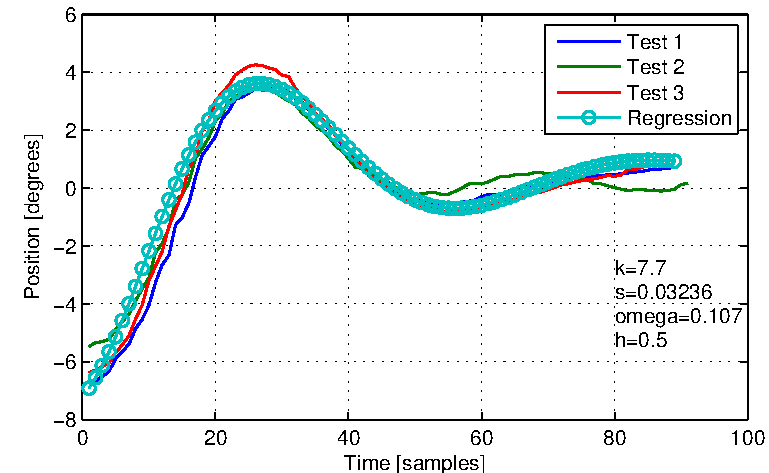
\includegraphics{plot/pbtest}
	\caption{Pitch test with Vicon, Bow pushed down.}
	\label{fig:pbtest}
\end{figure}
\begin{figure}[H]
	\centering
	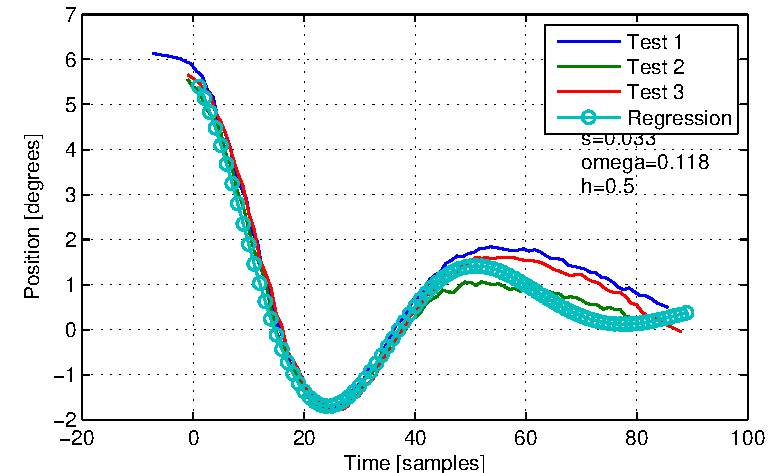
\includegraphics{plot/pstest}
	\caption{Pitch test with Vicon, Stern pushed down.}
	\label{fig:pstest}
\end{figure}

\newpage
\subsubsection{Roll test}
\begin{figure}[H]
	\centering
	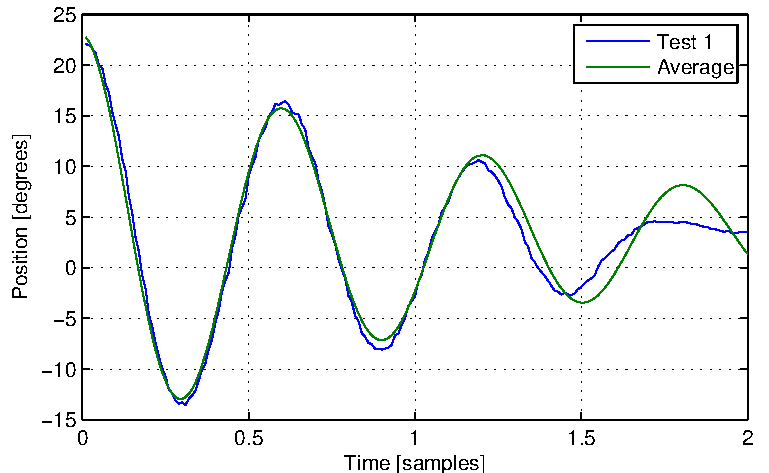
\includegraphics{plot/rltest}
	\caption{Roll left test with Vicon, Port side pushed down.}
	\label{fig:rltest}
\end{figure}
\begin{figure}[H]
	\centering
	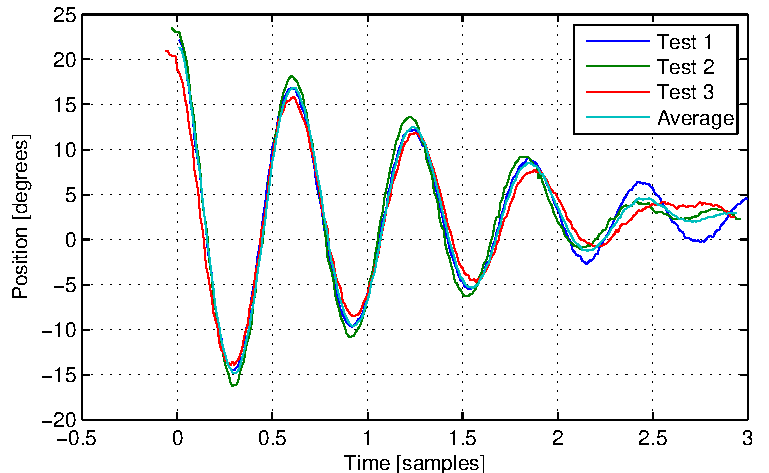
\includegraphics{plot/rrtest}
	\caption{Roll right test with Vicon, Starboard side pushed down.}
	\label{fig:rrtest}
\end{figure}


The rigid body constants for the vessel can be found in table \ref{tab:constants} and the results from measurements and estimation can be found in table \ref{tab:dmatrix}.
\todo{Disse skal måles op og sættes ind}
\begin{table}[htbp]
\centering
\begin{tabular}{ccc}
	\toprule
  Coefficient & Value \\
  \midrule
  $m$ & 13 \\
  $x_g$ & 0.03 \\
  $y_g$ & 0\\
  $z_g$ & 0.03\\
  $I_{xz}$ & -0.05359 \\
  $I_{zx}$ & -0.05359 \\
  $I_{xy}$ & -0.01260 \\
  $I_{yx}$ & -0.01260 \\
  $I_{yz}$ & -0.00108 \\
  $I_{zy}$ & -0.00108 \\
  $I_z$ & 1.10675 \\
  $I_y$ & 1.08921 \\
  $I_x$ & 0.06541 \\
  \bottomrule
\end{tabular}
\caption{Rigid body mass matrix constants for $M_{RB}$}
\label{tab:constants}
\end{table}

\begin{table}[htbp]
\centering
\begin{tabular}{ccc}
	\toprule
  Hydrodynamic\\Coefficient & Value \\
  \midrule
  $X_u$ & 2.86 \\
  $Y_v$ & 32.5 \\
  $K_v$ & -0.975 \\
  $N_v$ & 0.975 \\
  $N_r$ & 0.26285 \\
  $Y_r$ & 0.09263 \\
  $K_r$ & 0.01273 \\
  $Y_p$ & -0.00503 \\
  $K_p$ & 0.00084 \\
  $N_p$ & -0.00069 \\
  $M_q$ & 0.0712 \\
	\bottomrule
\end{tabular}
\caption{Results of fitted values and the calculated coefficients.}
\label{tab:dmatrix}
\end{table}

\begin{table}[htbp]
\centering
\begin{tabular}{ccc}
	\toprule
  Restoring force\\Coefficient & Value \\
  \midrule
  $K_\varphi$ & 0.0007 \\
  $M_\theta$ & 0.0150 \\
  	\bottomrule
\end{tabular}
\caption{Results of fitted values and the calculated coefficients.}
\label{tab:gmatrix}
\end{table}

This makes the linear damping matrix as:
\begin{align}
D = -
\begin{bmatrix}
2.86 & 0 & 0 & 0 & 0\\
0 & 32.5 & -0.00503 & 0 & 0.09263\\
0 & -0.975 & 0.00084 & 0 & 0.01273\\
0 & 0 & 0 & 0.0712 & 0\\
0 & 0.975 & -0.00069 & 0 & 0.26285
\end{bmatrix}
\end{align}
and the restoring for matrix as:
\begin{align}
G = -
\begin{bmatrix}
0 & 0 & 0 & 0 & 0\\
0 & 0 & 0 & 0 & 0\\
0 & 0 & 0.0007 & 0 & 0\\
0 & 0 & 0 & 0.0150 & 0\\
0 & 0 & 0 & 0 & 0
\end{bmatrix}
\end{align}
and the rigid body matrix as:
\begin{align}
M_{RB} =
\begin{bmatrix}
13 & 0 & 0 & 13\cdot0.03 & -13\cdot0\\
0 & 13 & -13\cdot0.03 & 0 & 13\cdot0.03\\
0 & -13\cdot0.03 & 0.06541 & -0.01260 & -0.05359\\
13\cdot0.03 & 0 & -0.01260 & 1.08921 & -0.00108\\
-13\cdot0 & 13\cdot0.03 & -0.05359 & -0.00108 & 1.10675
\end{bmatrix}
\end{align}
\section{Discussion}


\section{Conclusion}


\chapter{Bollard Pull}
\label{app:bollpull}

\section{Objective}
The purpose of this measurement journal is to test if the force, which is generated from the vessel, is linear with the control input to the thrusters or if there should be a mapping between these.

\section{Theory}
If the linear stepped input to the thrusters ends out in a linear output of the vessel it can be approximated that the translation from input to output is linear. This makes some of the controlling of the vessel less complicated due to the non existing non linear mapping from input to output. If a mapping is needed this needs to be taken care of in the control of the vessel, which needs to be compensated at least in the simulations of the vessel. This makes it possible to take it into account in the plant model of the vessel but might be neglected in the control model.

\section{Tools}
\begin{table}[htbp]
\centering
\begin{tabular}{ccc}
	\toprule
  Tool \\
  \midrule
  Test vessel \\
  Dynamometer \\
  Rod to apply on the vessel \\
  	\bottomrule
\end{tabular}
\caption{Tools needed to test the forces generated by the vessel.}
\label{tab:bollpulltool}
\end{table}

\section{Method}
The first tests, utilizing the thrusters forward, was performed by applying a rod symmetric at the stern of the vessel. The rod was extended such that it was possible to measure the force generated by the vessel from the bay, while the vessel was in the middle of the lake. This is done to make the reflecting waves as little as possible. The same procedure are used when testing the vessel while thrusting backwards. The test setup can be seen on figure .

\begin{figure}[htbp]
	\centering
	\includesvg[width=0.6\textwidth]{bollpullsetup}
	\caption{Setup while testing bollard pull, forward and backward motion.}
	\label{fig:bollpullsetup}
\end{figure}


\section{Results}
\begin{figure}[htbp]
	\centering
	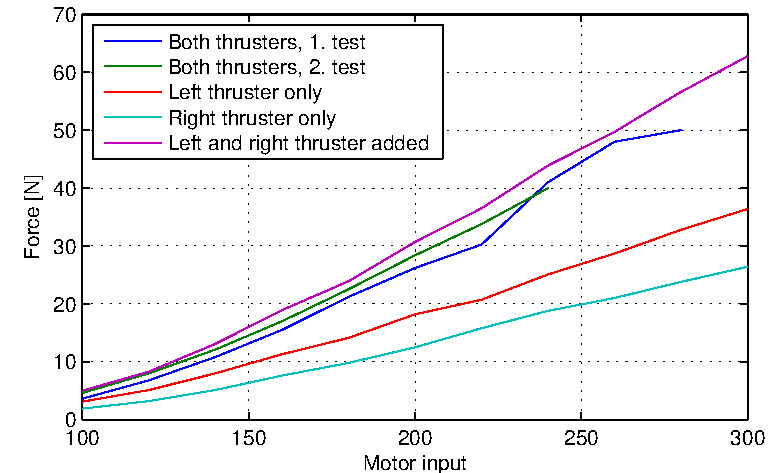
\includegraphics[width=0.6\textwidth]{plot/forwardthrust}
	\caption{Forward motion tests.}
	\label{fig:bollpullforward}
\end{figure}

\begin{figure}[htbp]
	\centering
	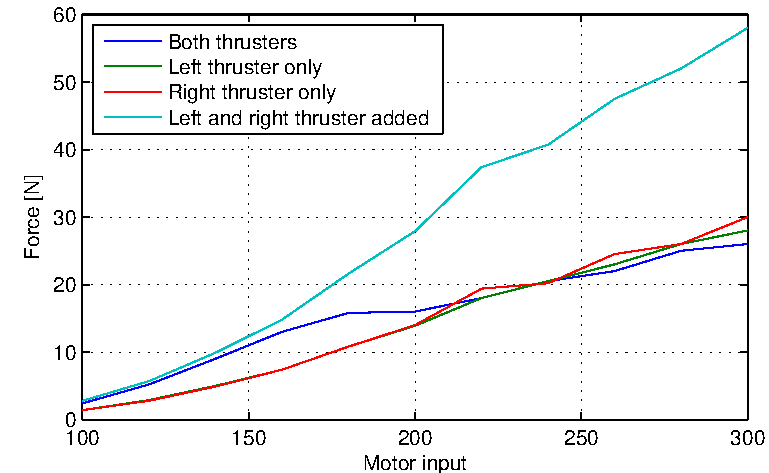
\includegraphics[width=0.6\textwidth]{plot/backthrust}
	\caption{Backward motion tests.}
	\label{fig:bollpullbackward}
\end{figure}

\begin{figure}[htbp]
	\centering
	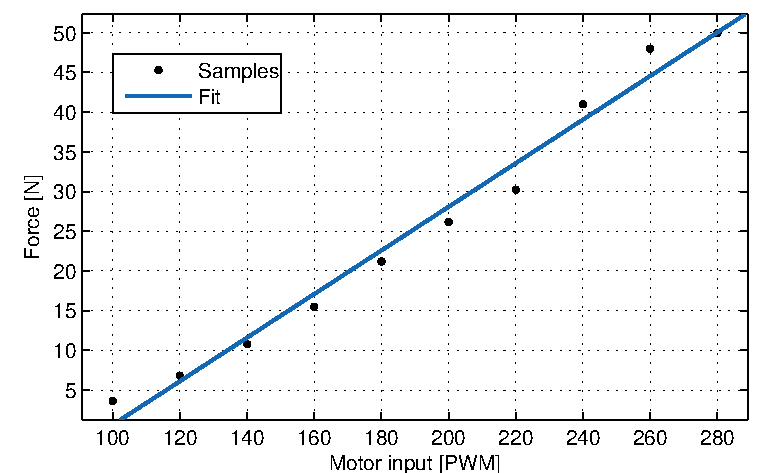
\includegraphics[width=0.6\textwidth]{plot/both_force_1_1order}
	\caption{Forward motion test with 1 order polynomial fitting.}
	\label{fig:1_1order}
\end{figure}

\begin{figure}[htbp]
	\centering
	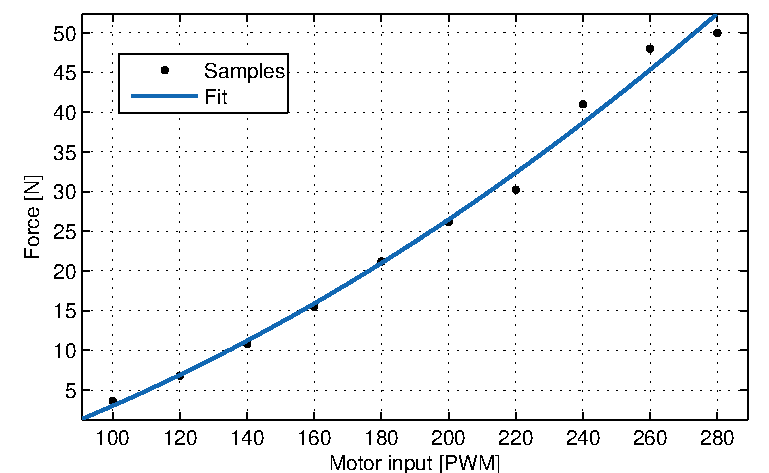
\includegraphics[width=0.6\textwidth]{plot/both_force_1_2order}
	\caption{Forward motion test with 2 order polynomial fitting.}
	\label{fig:1_2order}
\end{figure}

\begin{figure}[htbp]
	\centering
	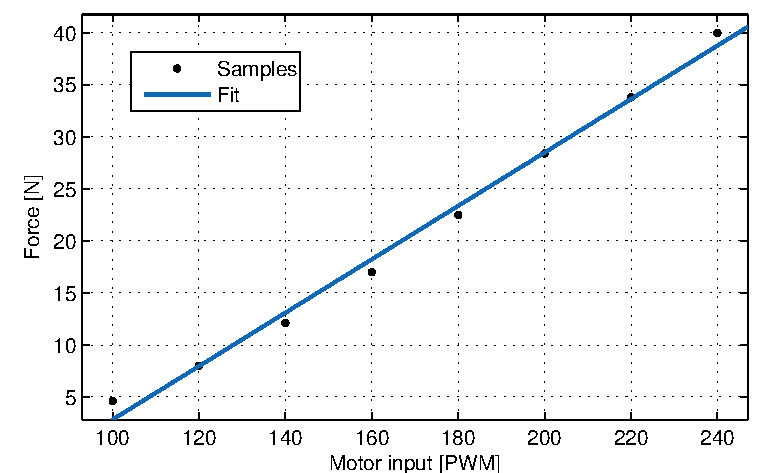
\includegraphics[width=0.6\textwidth]{plot/both_force_2_1order}
	\caption{Forward motion test with 1 order polynomial fitting.}
	\label{fig:2_1order}
\end{figure}

\begin{figure}[htbp]
	\centering
	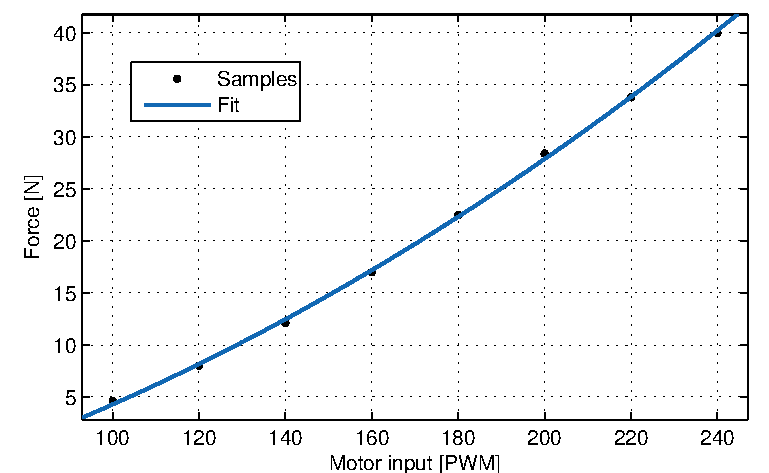
\includegraphics[width=0.6\textwidth]{plot/both_force_2_2order}
	\caption{Forward motion test with 2 order polynomial fitting.}
	\label{fig:2_2order}
\end{figure}

\begin{figure}[htbp]
	\centering
	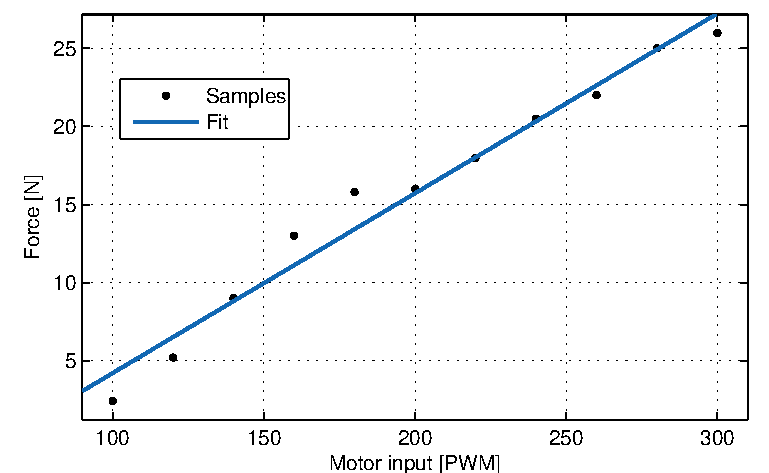
\includegraphics[width=0.6\textwidth]{plot/both_force_3_1order}
	\caption{Backward motion test with 2 order polynomial fitting.}
	\label{fig:3_1order}
\end{figure}

\begin{figure}[htbp]
	\centering
	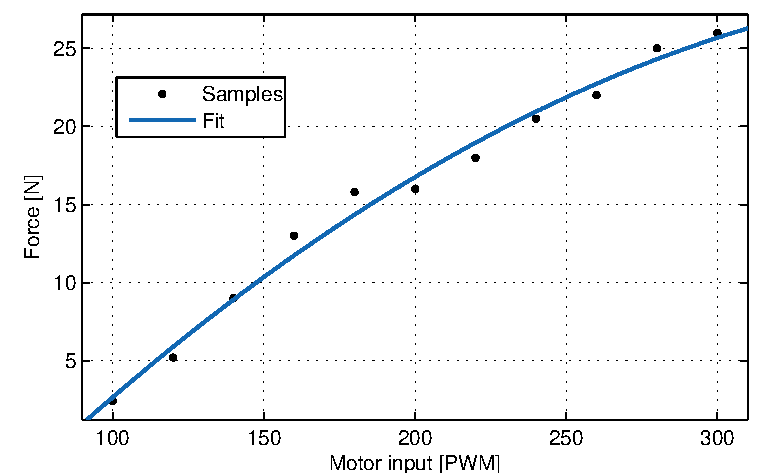
\includegraphics[width=0.6\textwidth]{plot/both_force_3_2order}
	\caption{Backward motion test with 2 order polynomial fitting.}
	\label{fig:3_2order}
\end{figure}

\begin{table}[htbp]
\centering
\begin{tabular}{cccc}
	\toprule
  Test & $R^2$ & RMSE & Function\\
  \midrule
  Both thrusters, forward \ref{fig:1_1order} & 0.9824 & 2.3626 & $f(x)=0.2746\cdot x-26.84$\\
  Both thrusters, forward \ref{fig:1_2order} & 0.9906 & 1.8414 & $f(x)=0.0004976\cdot x^2+0.08552\cdot x-10.52$\\
  Both thrusters, forward \ref{fig:2_1order} & 0.9929 & 1.1513 & $f(x)=0.2567\cdot x-22.83$\\
  Both thrusters, forward \ref{fig:2_2order} & 0.9994 & 0.3638 & $f(x)=0.0005208\cdot x^2+0.07958\cdot x-8.875$\\
  Both thrusters, backward \ref{fig:3_1order} & 0.9729 & 1.345 & $f(x)=0.1152\cdot x-7.318$\\
  Both thrusters, backward \ref{fig:3_1order} & 0.9883 & 0.9383 & $f(x)=-0.0002593\cdot x^2+0.2189\cdot x-16.65$\\
  \bottomrule
\end{tabular}
\caption{Coefficient of determination, Root Mean Square Error and the functions to the fittings.}
\label{tab:fitting}
\end{table}

\section{Discussion and conclusion}
The fitting maps from motor \ac{PWM} input to force output in $N$. When looking at the two first regressions at the forward motion it can be chosen to either use the first order fitting or the second order fitting. The coefficient of determination and the RMSE does not deviate much from the samples in either cases. Thus it is concluded that the first order fitting can be as good as the second order fitting, and the first order is chosen as fitting.

When looking at the regression for the backward motion it can be seen, that the second order fitting estimates the $a$ coefficient of the fitting to be negative. This is due to the backward test. At a \ac{PWM} input above 160 is applied, the vessel starts to ventilate from the propellers. This makes the force, which the vessel's pulls with, be lesser than it actually would if it did not ventilate. Therefore is the first order also seen as the most reliable while going backwards.

\chapter{Verification of attitude with a camera}
\head{This is a description of a technique to verify an attitude
estimator by using a camera. It utilizes the horizon as the reference.}

\section{Purpose}
\section{Method}


While testing it is of importance to make some verifications. When implementing an attitude
estimator for pitch and roll, it is hard to verify that it works as
intended. A simple way to test it is to put the sensor in positions
that can be measured in a static environment, that is by i.e. putting
in on a table on what is to be defined as flat, then angle it
some known degrees and see if the estimator agrees.

Depending on how exotic the estimator is, it might utilise a dynamic
model, in an attempt to improve the accuracy of the estimates. This is
harder to measure in the static lab setup. Another way is to record
the attitude with another setup that is known to work, but that could
not exist, hence the need to implement a new one. Alternatively a
camera can be used, and this is the method to be described in the
following.

One could also use a visual means of determining the heading. The idea
here is to mount a camera on the rigid body object containing the
sensor in the longitudinal direction of the axis of interest. That is
a camera pointing forward for the roll determiniaton or a camera
pointing to one side for the pitch determiniaton. This is intended for
use on ships.

This method relies on a known reference, that is stationary or at least
known at all time. The most ideal scenario is to be in open water
where the horizon is between the sea and the sky. This is guaranteed
to be horizontal, giving us an absolute reference to compare against.

In a non ideal scenario is to e.g. use the harbour quay. This works if
the ship is not moving a lot around relative to the quay, else you
need to know the exact position to the quay to determine the angle the
camera should see as zero. This is also possible but is out of scope
of this description.

\missingfigure{Screenshot of the images generated}

\documentclass[a4paper,11pt,oneside,fleqn]{article}
% Pakker
\usepackage[utf8]{inputenc} % Så må vi bruge æ, ø og å
%\usepackage(ansinew){inputenc}
%\usepackage(danish){babel} % Dansk opsætning
\usepackage[T1]{fontenc} % Hjælper med orddeling ved æ, ø og å. Sætter fontene til at være ps-fonte i stedet for bmp.
\usepackage[english,final]{varioref} % Vi kan anvende \vref
\usepackage{array,booktabs} % Til gode tabeller
\usepackage[printonlyused,withpage]{acronym} % Smart akronymhåndtering
\usepackage{minitoc} % Vi kan lave del inholdsfortegnelser forhåbentlig
\usepackage{graphicx} % We can now use \includegraphics and stuff
\usepackage[svgnames]{xcolor} % Colored stuff i.e. \colorbox
\usepackage{pdfpages} % Inkludere en pdf side som en side  
\usepackage{amsmath,amsfonts,amssymb} % God matematik
\usepackage{wasysym}% smileys
\usepackage{textcomp} % More text stuff, such as numero
\usepackage{mathtools} % We can now use \xRightarrow{hello world}
\usepackage{booktabs} % Rulers for tables
\usepackage[thinspace,amssymb]{SIunits} % Using macros for typesetting SI units
\usepackage{natbib} % Use proper citation
\usepackage{tocbibind} % Includes toc and bib in toc
\usepackage{listingsutf8} % Code listings
\usepackage{tabularx,booktabs} % Tables with fixed width
\usepackage{todonotes} % Todonotes
\usepackage{tcolorbox} % Colored boxes!
\lstset{extendedchars=\true, inputencoding=utf8/latin1} % This and listingsutf8 makes us able to use utf8 and latin1 as inputfiles
\lstset{language=matlab,frame=single,basicstyle=\footnotesize\ttfamily}
\usepackage[pdftex]{hyperref} % Hyperlinks
\hypersetup{backref,
bookmarks=true,
bookmarksnumbered=true,
colorlinks=true,
linkcolor=Navy,
citecolor=Green} % Setting some fancy colors
\DeclareUnicodeCharacter{00A0}{~} % Fix odd OSX/textwrangler no break space charater
\newcommand{\head}[1]{\vspace{3mm}{\noindent \hspace{-0.5em} \fcolorbox{gray}{GhostWhite}{\parbox[c]{\textwidth}{\slshape{#1}}}\vspace{2mm}}} % Header

\let\oldhat\hat
\renewcommand{\vec}[1]{\boldsymbol{#1}}
\renewcommand{\hat}[1]{\oldhat{\mathbf{#1}}}

\newcommand{\MATLAB}{M{\footnotesize ATLAB}}

\begin{document}
% Frontpage
\author{Nick Østergaard}
\title{Users Manual\\
	for\\
\emph{ASV Formation Control for Surveying Purposes}}
\date{\today}
\maketitle
\thispagestyle{empty}
\begin{center}
	\includegraphics[width=13cm]{fig/aauship}
\end{center}
\vfill
\begin{center}
	
\includegraphics[width=5cm]{fig/AAU_LOGO_CMYK_UK}\\
	Department of Electronic Systems
\end{center}
\clearpage

% Abstract
\begin{abstract}\addcontentsline{toc}{section}{Abstract}

This report documents the design and implementation of optimal control
of a helicopter test setup controlling the travel and elevation with
and without feedback using a linear quadratic controller.

The helicopter model has 3 degrees of freedom, controlled by two
horizontal propellers to adjust pitch and elevation, nonzero pitch
makes it travel.

The implementation is done in \MATLAB\ and with QuaRC from Quanser
integrated with Simulink and MathWorks' Real-Time Workshop. The code
and simulink models are also presented in the appendix.
	
\end{abstract}


% Table of contents
\tableofcontents
%\listoftables
%\listoffigures
\newpage

% Inclusion of body text here
\chapter{Introduction}
\head{In this chapter is the motivation for the project stated and the previous work within the subject will be summed up.}

\section{Motivation and the AAUSHIP Project}
The Port of Aalborg would like Aalborg University to help them to expand their options of improving the conditions of the Limfjord. One of their tasks is to map the seabed of the Limfjord to get bathymetry data. This will help them guide larger cargo ships to port while using the autonomous ships as guidance.

Another aspect from The Port of Aalborg is a task to escort larger ships with cargo into The Port of Aalborg. This is done by a pilot whom needs to sail out to incoming larger cargo ships and escort them safely into port. The pilot does this in a pilot boat which is controlled manually by the pilot. The Port of Aalborg would like this process to become autonomous such that an autonomous boat can sail to the cargo ship and to some extend take over the control and guide the cargo ship into port. The system to do this implies that The Port of Aalborg needs an autonomous ship which can perform this task.

The mapping itself can be done by one ship or by more. For the moment one of the ships from The Port of Aalborg, which is manned, and covers the mapping of the closer part of the Limfjord ($\approx$ 65 km). This is only done every third year, but mapping around Hals Barre (a sandbar \todo{slet efterfølgende kommentar igen engang}and not a beach bar) at the end of the Limfjord is a more critical place and is mapped every third month.

If The Port of Aalborg had an autonomous ship fleet at their disposal, which could sail out and do the mapping autonomously, they would get updated bathymetry maps with a higher update frequency than they have currently \citep{portofaalborg}. This will result in a digitalizing of the seabed, a digital map, which has different implementation options by The Port of Aalborg.

This thesis will utilise formation control and extensions to manoeuvre agents through a specified area for surveying purposes. The aspect of formation control is chosen due to the rather large areas that The Port of Aalborg needs so cover. When applying formation control it is assumed to be faster to cover a larger area than if one single boat needed to scan the area. The formation that are to be chosen depends on the specific area of interest, which could e.g. be inside the harbour or around the pillars of the bridge. Chapter~\vref{ch:formcontrol} will introduce what kind and scopes of formation control that exists today. These theories makes the basis for the formation control within the scope of this project.

As a future scope this can be used when making a model of the seabed of how this will get sanded. This model can tell The Port of Aalborg when to go clean the seabed. The AAUSHIP project can be used to verify this model, such that The Port of Aalborg do not have to go out with equipment to solve the sanding without the need of it.

\section{The Mission}
\label{sc:mission}
Within the scope of this project the robots will be unmanned ships,
\ac{ASV}. The ship's main purpose will be to map the seabed by using
sonars to obtain bathymetry data. When one ship need to do this alone, and due to the range of
the sonar, the time spend could be improved by using multiple ships. The sonar scanning would
be done as seen on figure~\vref{fig:concept-art}.

\begin{figure}[htbp]
	\centering
	\subfloat[One ship\label{fig:concept-art1}]{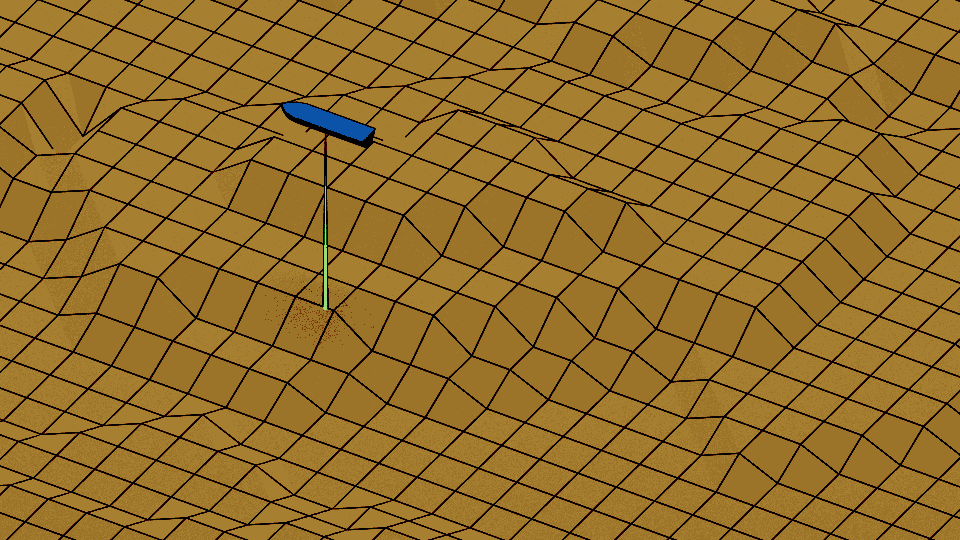
\includegraphics[width=0.48\textwidth]{fig/conseptart-single}}
	\ % One forced space to seperate figures
	\subfloat[Thee ships\label{fig:concept-art3}]{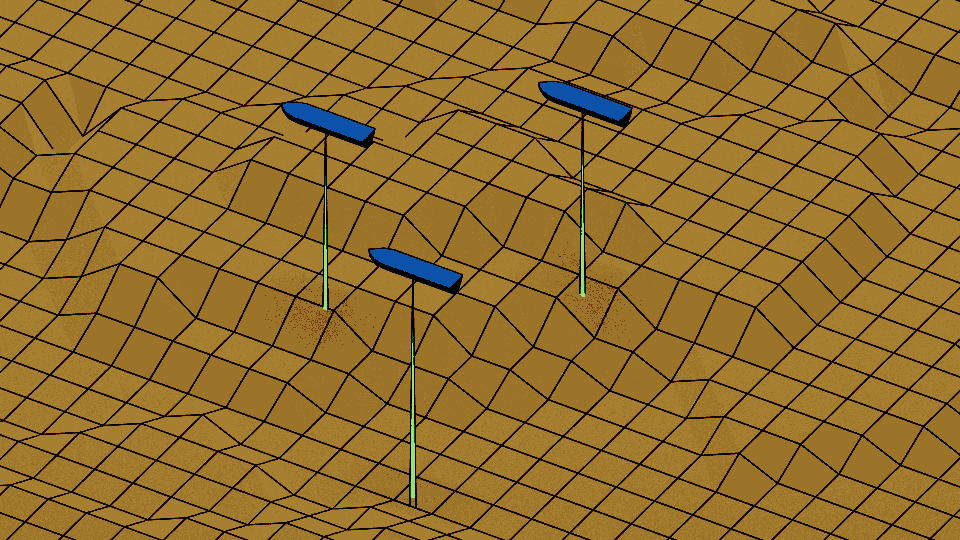
\includegraphics[width=0.48\textwidth]{fig/conseptart-formation}}
	\caption{Comparison of two ways to cover an area with a lawn mower
	pattern.}
	\label{fig:concept-art}
\end{figure}

When only one ship (figure~\vref{fig:concept-art1}) need to map a complete seabed this process could
take up much time dependent on the area that need to be covered. The
time spend could be improved to make this mapping more efficient. One
way of optimizing the time used is to add more ships (figure~\vref{fig:concept-art3}) to help map the
seabed. To make the process of this as optimal as possible it could be
of benefit to implement formation control in the specific assignment.

I cooperation with the port of Aalborg, a use case is presented, where we can perform tests of the platform, and use those to compare the performance of our system to their system.
\begin{figure}[htbp]
	\centering
	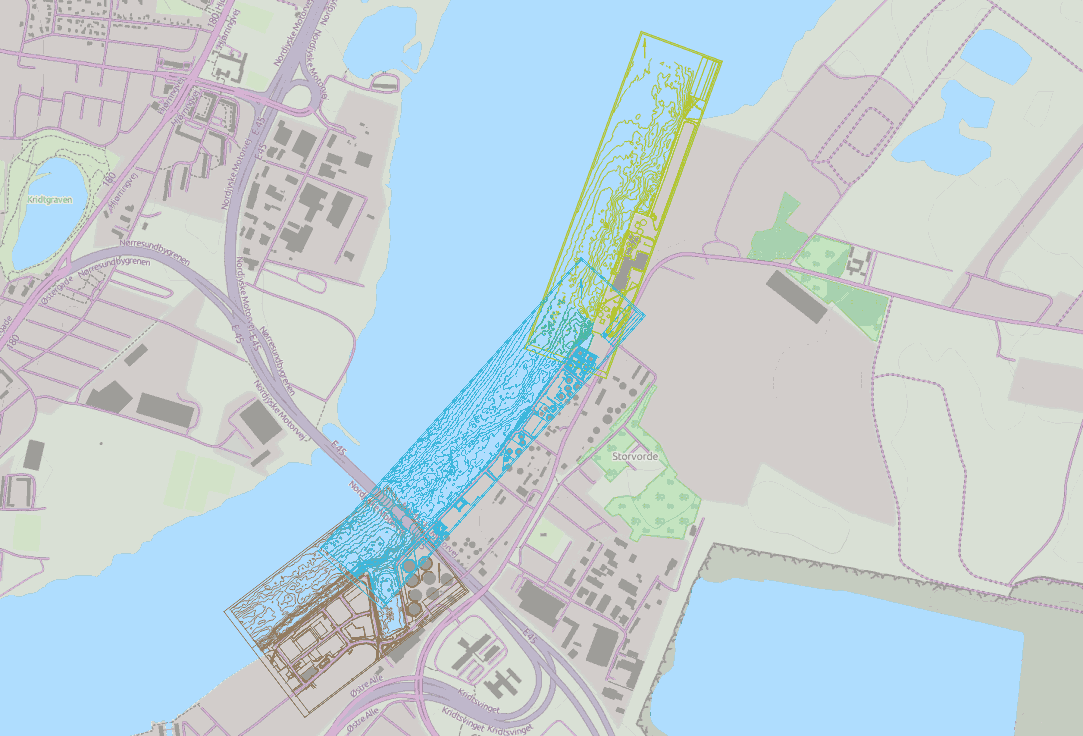
\includegraphics[width=\textwidth]{fig/use-case-data}
	\caption{Area of the harbour at Aalborg Portland provided as sample
	data from Aalborg Havn. Background map data CC BY-SA OpenStreetMap.}
	\label{fig:diffforms}
\end{figure}

When performing this kind of surveying with multiple ships, it is important to take note of the kind of sensor it uses and the coverage that it provides. Initially the port of Aalborg used single beam echo sounders, but have in recent years turned over to multibeam sonars for their survey boat, which has improved their resolution and time for a survey. But they still wishes to improve the survey update rate, by e.g. using fairly low cost autonomous ships to get better indication of the seabed to identify if an expensive thorough survey is needed. An image of the survey vessel they use now used can be seen on figure \ref{fig:alba}. As it can be seen, this survey vessel is relatively large, being over 20 metres long. To comparison is the AAUSHIP only 1.1 metres long. For surveying in smaller areas, like inside the harbour area, Aalborg Havn uses a smaller scale vessel which is 12 metres long. This vessel is only used at the smaller areas thus not the one being used out in the Limfjord close to Aalborg.
\begin{figure}
	\centering
	\includesvg{alba}
	\caption{The survey vessel used by Aalborg Havn named Alba.}
	\label{fig:alba}
\end{figure}



%This could be done in several ways, but is mostly thought of in a
%rigid formation, such that the formation maps the same area of the
%seabed the whole time. The idea can be seen on
%figure~\vref{fig:concept-art}.

\section{Objective}

\head{This section describes what can be done for humanity by the use of
automation in the realm of Aalborg.}

A use case that is a basis of this project is a service that surveying
companies offer, which is to survey and map the seabed of waterways and
lakes. Currently they do this very manually my sailing with a boat in
the lake after a \ac{GNSS} in the boat. In waterways as small rivers
and the like in Denmark they do it by a smaller boat or raft, where
they are using a prism system and a stick to take point measurements
of the river.

These tasks could be automated and probably improve surveying time by
using an autonomous system that can cover this. Here focus is on
trying to design such a system with small ships sailing in formation
to scan a predefined area.

This will then lead to defining the needed capabilities for
the formation control.

\todo{See 3.3.2 in \citep{thorvaldsen} for some nice definitions.}

\chapter{General formation control}
\head{This section will give a short introduction to formation control in general, by discussing existing formation control paradigms and relating them to the motivation of the AAUSHIP as a survey platform consept.}

%\head{Formation control in general is concerned with simultaneous control of dynamic systems. These systems is often referred to as agents where the objective of these is to maintain a static reference to a specified object. This object could be another agent witch then would be referred to as the leader. The other agents objective will then be to stay in the relative position to the leader within a static formation.}

The theory of formation control in general is widely applied. It is usually applied in assignments regarding control of robots which needs to be placed relative to each other. Depending on the given task of the robots, and which type of robots are in focus, the formation can be utilized in different ways \cite{muv-survey1}.

The robots can also be of various types: Driving vehicles, helicopters, aeroplanes, ships etc. which can be both manned and unmanned. The tasks that these robots needs to fulfill can vary greatly. Robots in groups in general have many purposes such as vacuum cleaning robots, who needs to clean a rather large area or flying swarm robots like quadcoptors who can make different kinds of assignments. When quadcoptors work as a combined group they could lift a certain amount of payload to achieve their goal as a group, or they could work individually in a network to do several smaller tasks. An example of how quadcoptors are working together can be examined at \citep{ethswarm}.

All the robots in the terminology of \cite{muv-survey} are called \textit{agents}. These agents move either individually or in formation. This formation can be rigid or be flexible. If the agents move in rigid formation they will keep their relative positions to each other and must not diverge from the formation. The formation could also be flexible which sometimes is preferable. If the distances between three agents on line are large, and an obstacle needs to be avoided, only one of the agents needs to move from this obstacle if the formation is flexible. This can be seen on figure~\vref{fig:form_avoid_right}.
\begin{figure}[htbp]
	\centering
	\includesvg[width=0.5\textwidth]{form_avoid_right}
	\caption{A flexible formation where the right agent avoids an obstacle.}
	\label{fig:form_avoid_right}
\end{figure}

\section{State of the art}
When looking into formation control many different types of control can be taken into control. The main types of formation control are separated into six different types, separated by \cite{muv-survey}, all under the main topic \textit{multiple vehicles coordination strategies}. The overview for this can be found in the survey paper \cite{muv-survey} who explains the six main types and a few alternations of these.

The theoretical views on control of \ac{MUV}'s behaviour are by \cite{muv-survey} divided into two classes; centralized and decentralized systems. If the system is centralized this means that all control of the formation is done on one agent, and the others receive information from the core agent. This form of system has the advantage that the core agent can optimize vehicle coordination, accommodate individual agent faults and monitor the accomplishment of the mission. The main disadvantage of this system is that if a fault should occur in the core agent this will affect and facilitate a failure of the whole system.

The opposite way of controlling the system would be in a decentralized way. This way of controlling the formation is inspired by the aggregation of birds and fish. This makes each agent able to communicate and share information in between. This means that each agent is given its own part of the complete objective and thus can only complete a part of it, like moving around an object to get to end point of a trajectory. The advantage is that faults in a single agent can be overlooked, thus more robust to faults, but can result in a less efficient objective outcome. A decentralized system may be more appropriate to scale up such that more agents can be included and the computational load can, in difference from the centralized system, be split up onto more agents.

The different types of coordination and control algorithms within centralized and decentralized systems include: \textit{behavioural-based}, \textit{virtual structure}, \textit{leader-follower}, \textit{graph-based} and \textit{potential field approaches}. Within these structures are the terms \textit{cooperation control} and \textit{formation control} used. Cooperative control focuses on the global task that the group of agents needs to fulfil, and the formation control is the actions performed by each agent which is shared with the other agents in the group. 
\begin{description}[style=nextline]
	\item [Virtual structure]
	In a virtual structure is the entire formation treated as a single entity. The behaviour coordination for a group of agents in a virtual structure is uncomplicated compared to the coordination of many agents, due to the making of one structure e.g. based on fixed distances between the agents. The disadvantage falls on the centralization due to the structure treated as a single entity. If a failure in this structure happen results in a failure in the entire structure.
	\item [Behaviour Based Methods]
	The behavioural based model employs several behaviours for each of the agents and the final control used to control the formation is derived from a weighting of the relative importance of each of the behaviours. This could for instance be navigational behaviours to enable a navigation to be the main goal while avoiding hazards and stay in formation. So if one agent needs to avoid a collision with an obstacle the rest of the group should not take this into account. Only that single ship needs to leave the formation and get back into formation again.
	\item [Leader-Follower Approaches]
	Applying leader-follower methods designates one agent as being the leader and the rest of the agents as followers. The following agents need to position themselves relative to the leader and maintain a desired relative position to the leader. This makes the simplicity to this method, but there is no feedback from the followers to the leader and thus makes that a disadvantage. Separation-separation and separation-bearing are two popular leader-follower formation controls, where the followers stay at specified separation and bearing from their designated leader. Within this method it is possible to split the group up into several smaller groups with their individual designated leader.
	\item [Potential Field Approach]
	Potential field approaches assigns potentials to agents to make a weighting between them. This weighting could for instance determine the relative distances between the agents. This is usually used when following a virtual leader, such that this process is only made relative to the agents within the structure. This method can make ensure a collision free formation when every agent has been assigned their potential weighting respectively. In this method obstacles can be included and have assigned potentials as well. This will become an avoidance radius from the specific object.
	\item [Graph Theory Approaches]
	When applying the graph theory method one assign every agent as a node and assign connections between the nodes. In graph theory this is denoted vertices and edges. The study with graph theory is mainly concentrated of the formation itself and related to changes within the structure. This can be related to the structure within a tree-structure which is used when assigning the formations in graph theory manor. This can be applied as communication analysis for the agents and consensus analysis can be of benefit. The edges between the nodes symbolizes the possible connections thus communication between them. The nodes that are connected are denoted as neighbours and are capable of communicating.
\end{description}

\subsection{Approaches on formation control}
When performing this kind of surveying with multiple ships, it is important to take note of the kind of sensor it uses and the coverage that it provides. Initially the port of Aalborg used single beam echo sounders, but have in recent years turned over to multibeam sonars for their survey boat, which has improved their resolution and time for a survey. But they still wishes to improve the update rate, by i.e. using fairly low cost autonomous ships.

\missingfigure{Picture of the port of Aalborg's survey boat.}

This does not have any relevant impact of how the mappings of the seabed would be due to the subsequent processing of the collected data from the maps.

Different formations of ships can be seen on figure~\vref{fig:diffforms}.
\begin{figure}[htbp]
	\centering
	\includesvg[width=0.5\textwidth]{diffforms}
	\caption{Different formations which the \ac{ASV}s can make.}
	\label{fig:diffforms}
\end{figure}

The formation of the ships may not need to be strictly rigid. Situations could appear where it would be of benefit to change the ship's formation. If the formation need to avoid an obstacle and one or more ships needs to go faster or slower, which leads to a change in the formation, it might be of benefit to regroup the formation which is faster to reach. An example can be seen on figure~\vref{fig:avoid}.

\begin{figure}[htbp]
	\centering
	\includesvg[width=0.5\textwidth]{form_avoid}
	\caption{A formation needs to go around an obstacle where the inner most ship chooses the shortest path and the formation regroups.}
	\label{fig:avoid}
\end{figure}

When doing the formation control it is important to figure out what one
want to achieve, and depending on the strategy and the formation type
some things are to be considered as requirements regarding how the
formation should work. In this discussion lawnmower patterns are considered. In this work thee ships are considered for simplicity, but it should be extensible to n-number of ships. The lawnmower patterns will suit well for the mapping of a seabed where one or more ships are to sail from shore to shore in a fjord.

\subsubsection{Initialisation}
When looking at the specific task several things needs to be taken into account. When starting the mission, the ships may start at positions that is not in the desired formation. It might be of importance that the ships are in
formation when they start tracking the desired track. Therefore some
attention must be given on how to make the ships initialize this
formation. This is referred to as the group coordination task. An approach is to make the ships sail individually to the
starting positions with a speed that makes them hit their respectively starting points at
the same time. If one reaches its start point much earlier
than the other it must stop, which is not wanted because it then can
drift out of position again. This basically means that there exists an initialization
phase and a tracking phase. The start heading should of
course align with the path at the start point such that the path following can begin with zero error. The ships could also target their group formation before starting at time zero at the path. This will eventually make the initialization take longer time but ensure that the ships have made the group coordination task and are ready to start at the path.

Another issue to be considered is to ensure that no ship at
any point in time reaches a minimum speed that is necessary for the
ship to not drift out of formation. This could be a problem in corners
of the formation if a stiff construction, where the inner most ship
has to move slower, to accommodate the shorter distance on an inner
circle arc.

Faults like blackout on a ship could also be considered in the control
design. I.e. what happens with the formation when one ship faults in a
blackout. Should the rest of the formation stop, should the formation
still follow this drifting ship or should the mission simply terminate
when it is discovered that a ship has blackout. This is under the assumption that the formation is decentralized and every ship has its own control and is not controlled from a mother ship.

In the initialization phase it is also relevant to consider how the
ships should avoid each other if they are on the wrong side of each
other. If it is of benefit that a specific ship is at the most inner route, and is located at an outer position before the group coordination, this ship needs to cross the formation to get to the desired starting position. This initialization needs to be adjusted in the initialization phase to ensure that no ships collide.

\begin{figure}[htbp]
	\centering
	\includesvg[width=0.4\textwidth]{cornoring}
	\caption{Two ships initializing and following the path offset
		equally on each side, ships are constrained to sailing parallel
		and heading the same as path when projected onto the path. Blue
	dot is start of path. Fully drawn splines is initializing phase.}
	\label{fig:cornoring}
\end{figure}

On figure~\vref{fig:cornoring} is a simple path following performed
with two ships in a stiff formation with an equal distance from the
path. It illustrates four steps. In step \#0 the ships initializes a
random position near the start of the path being the group coordination task. At \#1 it is tracking the
path in formation, whilst still in formation. This is referred to as a formation coordination task. At \#2, the green
(right) ship is in a tight inner curve where it is important to
consider design of the path such that the capabilities of the ship is not
exceeded to stay in formation. At \#3 it is back to straight line path
following in formation. \citep{thorvaldsen}.

\begin{figure}[htbp]
	\centering
	\includesvg[width=0.6\textwidth]{form_rigid_90}
	\caption{Three ships in formation needs to make a 90\textdegree turn and stays in their relative positions and keeps the rigid formation.}
	\label{fig:form_rigid_90}
\end{figure}

When the ships needs to make a turn about something they can do it in many ways. On figure~\vref{fig:form_rigid_90} the ships keep their formation whilst turning about the object. When they reach the other side and have finished their turn, the ships have kept formation but the outer most ship has now become the inner most ship. The reason to turn like this could be that the inner most ship, the yellow ship, cannot turn as sharp as demanded to stay the inner most ship. Therefore, instead of turning the formation, they stay geometrically rigid.

\begin{figure}[htbp]
	\centering
	\includesvg[width=0.6\textwidth]{form_change_90}
	\caption{Three ships in formation needs to make a 90\textdegree turn and changes their relative positions.}
	\label{fig:form_change_90}
\end{figure}

As seen on figure~\vref{fig:form_rigid_90} the ships could have benefit of turning like this. This way of turning could cause trouble in the top of the turn, where the ships eventually will collide due to errors and the relative close distance to each other. This way could be altered a little such that the ships will turn like on figure~\vref{fig:form_change_90}. There the ships adjust their position and velocities to ensure that they will not collide, but they will therefore leave their formation shortly to return back into position again.

\subsubsection{Degree of Actuation}
The degree of actuation is a matter that sets some limitations on how
the path following can be made, and thus the methods available to
control the ships.

AAUSHIP is a ship, which means that is is not fully actuated in the
whole 3D space, but this is not needed since it is moving on a
surface. To be fully actuated it must be able to have controls for
surge, sway and yaw.

There are different ways of controlling, and a few could be:
\begin{description}[style=nextline]
	\item [Three or more controls]
	When having three or more control parameters it is said that the vessel is fully actuated. This way of controlling is usually used in low-speed manoeuvring and stationkeeping mostly by offshore \ac{DP} vessels.
	\item [Two controls and Trajectory-Tracking control]
	Trajectory-Tracking is done in a three \ac{DOF} system, $e(t)\in\mathds{R}^2\text{X}S$. It is done with two control inputs, $u(t)\in\mathds{R}^2$. This means that the control problem is underactuated which cannot be solved by linear control theory. A vessel under these terms is able to manoeuvre along a path with constant sideslip angle using only surge and yaw. This is the classic approach for path following.
	\item [Two controls and Weather-Optimal heading]
	When taking the weather conditions, and in general the environmental disturbances, into account, it is done as a mean of all the disturbances. This is used to stabilize the vessel regarding the position. It is done by making the heading depend of the change in the mean of the environmental disturbances.
	\item [Two controls and Path-Following control]
	The standard way by having two controls, being surge and yaw, and achieving path-following, is to define a 2-D workspace. This workspace is placed along the trajectory with along-track and cross-track vectors that are to represent the error to minimize. This is usually done by applying the \ac{LOS} path following controller that makes use of surge and yaw to accomplish the path following. This implies that a six \ac{DOF} system model needs to be internally stable such that only the two control inputs are used.
	\item [One control]
	This is only done with systems with three \ac{DOF} and is normally only used to stationkeeping.
\end{description}
\citep{fossen}

\subsection{Delimitations}
Within the scope of the AAUSHIP project will the focus be to apply and extend a leader-follower approach at the ships. This will include several tasks. The two main tasks will be to make a group coordination task and a formation coordination task. The group coordination task will be, as described earlier, an objective to get the ships into the desired formation before or exactly at the starting point of the path following. The formation coordination task will be to make a leader, virtual or not, follow a predetermined path set by waypoints. The path should be generated from waypoints placed on a map due to that the ship needs to travel over larger distances. This will make a waypoint based follower where the path will be generated between the placed waypoints.

The placement of the waypoints will be placed such that the ships need to surge along a lawnmower pattern, where the turns have a lower requirement of turn radius dependent on the surge velocity of the most inner ship. This is due to the drift if the inner ship looses too much velocity.

When applying the leader-follower approach it needs to be determined how the formation precisely should be set up. In this project is only one leader considered at a time. The rest of the ships will act as followers to the leader. The idea can be seen on figure~\vref{fig:l_f} where only one leader is represented with a single or more followers.
\begin{figure}[htbp]
	\centering
	\includesvg[width=0.6\textwidth]{lead_follow}
	\caption{A leader is always assigned and potential followers are following.}
	\label{fig:l_f}
\end{figure}
When the followers are in formation with the leader is only the leader who is following a specified trajectory. The other ships, the followers, only keeps their position relative to the leader. This makes the predetermined formation moving along the path relative to how the leader is following the path. The leader is autonomous as well as the followers, but the path following is only done at the leader and the followers maintains their relative positions to the leader.

If the leader diverges from the path, drifting to the left, this will result in the whole formation drifting to the left. This problem can be dealt with in different ways, e.g. the control could react fast enough to make the formation get back on track within a specified time, or some fault tolerance could be done from the whole system. If the leader diverges from the path it could make the formation stay at their respective headings within a time slot before actuating towards the leader.

The formation needs to take into account if it is of benefit to change leader. If some kind of obstacle makes the formation turn about it, it might come to benefit to change the leader which needs to be done on the fly. This entails a change in the group coordination and the ships needs to set their relative position and heading from another ship.

The configuration of the formation will be set up, as a start, with one leader and a single follower. The follower will be offset from the leader with a distance of five metres. This can be seen on figure~\vref{fig:l_f1}.
\begin{figure}[htbp]
	\centering
	\includesvg[width=0.4\textwidth]{lead_follow1}
	\caption{The leader with a follower offset by 5 metres radius.}
	\label{fig:l_f1}
\end{figure}
This will be a rigid formation that the ships needs to keep at all times. The change of leader will eventually be taken into account when the ships needs to turn. If the formation needs to turn clockwise about it might be of benefit to change the leader. 

The location to test and implementation the AAUSHIPs will be in the Limfjord. The optimum will be to make the formation go across the Limfjord and back in lawnmower pattern and make measurements of the seabed. Due to the location where it is presumed to have enough space, the formation is not of bigger importance to the mapping. The only important thing to include regarding the formation is that the ships needs to be able to turn around without loosing so much velocity such that they start drifting and offset the formation.

\section{Notation}
For convince this section defines notation that is used throughout
this manuscript.

\subsection{Reference Frames}
When working with dynamical systems that move in space, such as the
ship, it is convenient to work with different frames of reference, and
this means that a proper notation has to be used. 

\citep{fossen}

\begin{table}[htbp]
	\centering
	\begin{tabular}{llccc}
		\toprule
		    & & Forces and & Liner and          & Positions and  \\
		DOF & & moments    & angular velocities & Euler angles   \\ 
		\midrule
		1 & motion in the $x$ direction (surge)       & $X$ & $u$ & $x$ \\
		2 & motion in the $y$ direction (surge)       & $Y$ & $v$ & $y$ \\
		3 & motion in the $z$ direction (surge)       & $Z$ & $w$ & $z$ \\
		4 & rotation about the $x$ axis (roll, heel)  & $K$ & $p$ & $\phi$ \\
		5 & rotation about the $y$ axis (pitch, trim) & $M$ & $q$ & $\theta$ \\
		6 & rotation about the $z$ axis (yaw)         & $N$ & $r$ & $\psi$ \\
		\bottomrule
	\end{tabular}
	\caption{\cite{sname1950} notion for marine vessels, from
	\citep[table~2.1]{fossen}}
	\label{tab:sname}
\end{table}


\section{Preliminaries}
As a means to present the methodology used in this it is important
to use a terminology that is easy to understand and not conflicts too
much with the reaferences. There fore this sections will describe some
of those.

Firstly for formation control there is two main tasks that is in a
basic formation control setup, and as describen in \citep{thorvaldsen}
he uses two terms to describe the overall task \textit{Formation
Control Problem} as the  \textit{Group Coordination Task} which is the
task where it to make the group form the initial formation, and then
the \textit{Formation Mission Task} which is the task of moving the
formation on the desired path. \todo{Ligende illustration som fig 3.1
	fra \citep{thorvaldsen} her.}


\section{Parts list}
See table~\vref{tab:parts}.
\begin{table}[htbp]
	\centering
	\begin{tabularx}{\textwidth}{ll}
	\toprule
	\# &  Model \\
	\midrule
	2 & Graupner InIine 750 \\
	2 & Electronic Speed Controller \\
	2 & Propellers \\
	2 & Prop Shaft \\
	2 & Motor to prop shaft couplings 5mm\\
	6 & LiPo 3600 mAh 4S1P batteries \\
	1 & Intelligent Charge Port (ICP) \\
	1 & Raspberry Pi or similar \\
	1 & 4-split USB hub\\
	1 & Echosounder \\
	\bottomrule
	\end{tabularx}
	\caption{Mechanical parts for an AAUSHIP}
    \label{tab:parts}
\end{table}


\section{Power System}

The power source in AAUSHIP is chosen to be LiPo batteries, which is
a type of battery chemistry where the operator take great care in not damaging
the batteries. If care is not taken they might catch on fire, which
cannot easily be extinguished. This can of course be dangerous.

\subsection{Power Harness}
The power system on the ship consists of some somewhat convoluted
wiring harnessed loosely in the hull structures. An single line
diagram is therefor provided to give an overview of the system.

\begin{figure}[htbp]
	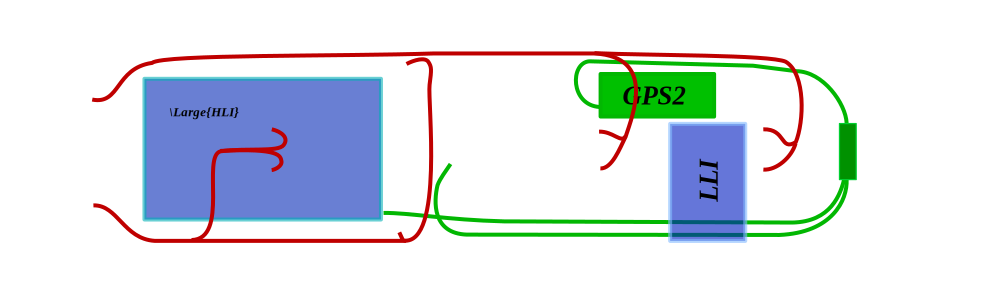
\includegraphics[width=\textwidth]{fig/harness}
\end{figure}

\subsection{LiPo Basics}
The LiPo battery packs each consists of four cells in series, which in
the LiPo battery world is called ``4S1P''. One parallel is what you get
when you only have a series connection.

Since each cell is normally not charged individually but across the
output terminals of the battery, every pack with more than one series
cell is equipped with a so called balance port. This is basically a
smaller multiple pin connector that has a connection to each cell,
such that is is possible for a ``balancer'' to discharge cells that is
unbalanced. An unbalanced cell is basically just a cell that does not
have the same voltage as the others.

This balancer is usually run whilst one is charging the main
connections. The purpose is to eliminate the difference that is
inherent in each cell not being exactly the same, such that one cell
does not get overcharged, when charging them in series.

\subsection{LiPo Battery Safety}
\begin{tcolorbox}[colback=yellow!75!,colframe=red]
It is strongly advised not to mess with the LiPo batteries before you
have read and understand how to handle them. A good resource for
learning some basics and safety about LiPo batteries are
\citep{tjintech:lipo-basics} and \citep{tjintech:lipo-safety}.
\end{tcolorbox}
 

\appendix
\chapter{Acronyms}
\label{ch:acronyms}
\begin{acronym}[TDMA]
%\begin{acronym}[HBCI]
	\acro{AAU}{Aalborg University}
  \acro{ASV}{Autonomous Surface Vessel}
	\acro{ADC}{Analog to Digital Converter}
  \acro{AHRS}{Attitude and Heading Reference System}
  \acro{BODY}{The body frame}
  \acro{CFD}{Computational Fluid Dynamics}
  \acro{DOF}{Degrees-Of-Freedom}
  \acro{DP}{Dynamic Positioning}
  \acro{ECEF}{Earth-Centered Earth-Fixed} 
  \acro{ECI}{Earth-Centered Inertial}
  \acro{EKF}{Extended Kalman Filter}
  \acro{FRF}{Formation Reference Frame}
  \acro{FRP}{Formation Reference Point}
	\acro{GNC}{Guidance, Navigation and Control}
  \acro{GNSS}{Global Navigation Satellite System}
  \acro{GPS}{Global Positioning System}
  \acro{GRS}{Ground Segment}
  \acro{HLI}{High Level Interface}
  \acro{IMU}{Inertial Measurement Unit}
	\acro{IP}{Internet Protocol}
	\acro{IPv4}{Internet Protocol version 4}
	\acro{IPv6}{Internet Protocol version 6}
  \acro{KF}{Kalman Filter}
  \acro{LKF}{Linear Kalman Filter}
  \acro{LOS}{Line-Of-Sight}
  \acro{LLI}{Low Level Interface}
	\acro{LSB}{Least Significant Bit}
  \acro{LTI}{Linear Time Invariant}
  \acro{MARG}{Magnetic, Angular Rate, and Gravity}
  \acro{MMSE}{Minimum Mean Square Error}
  \acro{MUV}{Multiple Unmanned Vehicle}
  \acro{MPC}{Model Predictive Control}
  \acro{NED}{North-East-Down}
  \acro{OSM}{OpenStreetMap}
  \acro{PWM}{Pulse Width Modulation}
  \acro{ROS}{Robot Operating System}
  \acro{RTK}{Real Time Kinematic}
  \acro{SOG}{Speed Over Ground}
  \acro{SSS}{Single Screw Ship}
  \acro{SSM}{State Space Model}
  \acro{TSS}{Twin Screw Ship}
  \acro{UGAS}{Uniformly Globally Asymptotically Stable}
  \acro{UGES}{Uniformly Globally Exponentially Stable}
  \acro{UGS}{Uniformly Globally Stable}
  \acro{UKF}{Unscented Kalman Filter}
  \acro{WGS84}{World Geodetic System 1984}
\end{acronym}



% Bibliography
\bibliographystyle{apalike}
\bibliography{bib}\label{sec:bibliography}

\end{document}


\backmatter
\bibliographystyle{apalike}
\bibliography{../manual/bib}
\label{ch:litt}

%\settocdepth{section}
\listoftodos
\end{document}

